\documentclass[twoside]{book}

% Packages required by doxygen
\usepackage{fixltx2e}
\usepackage{calc}
\usepackage{doxygen}
\usepackage[export]{adjustbox} % also loads graphicx
\usepackage{graphicx}
\usepackage[utf8]{inputenc}
\usepackage{makeidx}
\usepackage{multicol}
\usepackage{multirow}
\PassOptionsToPackage{warn}{textcomp}
\usepackage{textcomp}
\usepackage[nointegrals]{wasysym}
\usepackage[table]{xcolor}

% Font selection
\usepackage[T1]{fontenc}
\usepackage[scaled=.90]{helvet}
\usepackage{courier}
\usepackage{amssymb}
\usepackage{sectsty}
\renewcommand{\familydefault}{\sfdefault}
\allsectionsfont{%
  \fontseries{bc}\selectfont%
  \color{darkgray}%
}
\renewcommand{\DoxyLabelFont}{%
  \fontseries{bc}\selectfont%
  \color{darkgray}%
}
\newcommand{\+}{\discretionary{\mbox{\scriptsize$\hookleftarrow$}}{}{}}

% Page & text layout
\usepackage{geometry}
\geometry{%
  a4paper,%
  top=2.5cm,%
  bottom=2.5cm,%
  left=2.5cm,%
  right=2.5cm%
}
\tolerance=750
\hfuzz=15pt
\hbadness=750
\setlength{\emergencystretch}{15pt}
\setlength{\parindent}{0cm}
\setlength{\parskip}{3ex plus 2ex minus 2ex}
\makeatletter
\renewcommand{\paragraph}{%
  \@startsection{paragraph}{4}{0ex}{-1.0ex}{1.0ex}{%
    \normalfont\normalsize\bfseries\SS@parafont%
  }%
}
\renewcommand{\subparagraph}{%
  \@startsection{subparagraph}{5}{0ex}{-1.0ex}{1.0ex}{%
    \normalfont\normalsize\bfseries\SS@subparafont%
  }%
}
\makeatother

% Headers & footers
\usepackage{fancyhdr}
\pagestyle{fancyplain}
\fancyhead[LE]{\fancyplain{}{\bfseries\thepage}}
\fancyhead[CE]{\fancyplain{}{}}
\fancyhead[RE]{\fancyplain{}{\bfseries\leftmark}}
\fancyhead[LO]{\fancyplain{}{\bfseries\rightmark}}
\fancyhead[CO]{\fancyplain{}{}}
\fancyhead[RO]{\fancyplain{}{\bfseries\thepage}}
\fancyfoot[LE]{\fancyplain{}{}}
\fancyfoot[CE]{\fancyplain{}{}}
\fancyfoot[RE]{\fancyplain{}{\bfseries\scriptsize Generated by Doxygen }}
\fancyfoot[LO]{\fancyplain{}{\bfseries\scriptsize Generated by Doxygen }}
\fancyfoot[CO]{\fancyplain{}{}}
\fancyfoot[RO]{\fancyplain{}{}}
\renewcommand{\footrulewidth}{0.4pt}
\renewcommand{\chaptermark}[1]{%
  \markboth{#1}{}%
}
\renewcommand{\sectionmark}[1]{%
  \markright{\thesection\ #1}%
}

% Indices & bibliography
\usepackage{natbib}
\usepackage[titles]{tocloft}
\setcounter{tocdepth}{3}
\setcounter{secnumdepth}{5}
\makeindex

% Hyperlinks (required, but should be loaded last)
\usepackage{ifpdf}
\ifpdf
  \usepackage[pdftex,pagebackref=true]{hyperref}
\else
  \usepackage[ps2pdf,pagebackref=true]{hyperref}
\fi
\hypersetup{%
  colorlinks=true,%
  linkcolor=blue,%
  citecolor=blue,%
  unicode%
}

% Custom commands
\newcommand{\clearemptydoublepage}{%
  \newpage{\pagestyle{empty}\cleardoublepage}%
}

\usepackage{caption}
\captionsetup{labelsep=space,justification=centering,font={bf},singlelinecheck=off,skip=4pt,position=top}

%===== C O N T E N T S =====

\begin{document}

% Titlepage & ToC
\hypersetup{pageanchor=false,
             bookmarksnumbered=true,
             pdfencoding=unicode
            }
\pagenumbering{alph}
\begin{titlepage}
\vspace*{7cm}
\begin{center}%
{\Large My Project }\\
\vspace*{1cm}
{\large Generated by Doxygen 1.8.13}\\
\end{center}
\end{titlepage}
\clearemptydoublepage
\pagenumbering{roman}
\tableofcontents
\clearemptydoublepage
\pagenumbering{arabic}
\hypersetup{pageanchor=true}

%--- Begin generated contents ---
\chapter{Assignment 1\+: by Joseph Seklawy -\/ 12578845}
\label{index}\hypertarget{index}{}The task is to simulates the generation of data from several sensor(rangers) types, and performs data fusion.

Users will have to initiate the sensors they wish to use within the main and then using the varius set functions available in the \hyperlink{ranger_8h_source}{ranger.\+h} class header, they can then set the various parameters they wish to change. These sensors should then be passed into a vector which itself is passed to the \hyperlink{classRangerFusion}{Ranger\+Fusion} class constructor. Once the code is run, the user will be prompted to input the number of cells they wish to create to be checked by the sensors created beforehand. The sensors will then randomly generate data based on the inputed variables and its specifications, and that data will be run through the Graband\+Fuse\+Data function which determines based on the sensor readings whether a cell is free, occupied or unkown. This is achieved in a few ways depending on the sensor. Much of the implementation for the following is found within the \hyperlink{analysis_8h}{analysis.\+h} header and its coressponding analysis.\+cpp file.

For laser sensors, the process for determining cell states is rather simple. For example, a laser with a F\+OV of 180 degrees and a angular resolution of 30 degrees will produce 8 readings, starting from 0 degrees and incrementing by 30 till reaching 180. Since the length of each reading is known and the angle from a specfic reading and the x axis can be found, the coordinates for each reading can be found by splitting the vector into its vertical and horizontal components. From here its a simple case of checking wether these coordinates exists within the bounds of a cells sides, which can be found since the cell centre and side lengths can be obtained from the cell class. If this case proves true then the cell is O\+C\+C\+U\+P\+I\+ED. A cell is F\+R\+EE if the line between the laser centre and its reading passed through the sides of a cell but D\+O\+ES N\+OT stop within the cell itself. This can be determined using a line intersection algorithm.

In the case of a sonar, the check is a little more complicated. For a cell to be determined as O\+C\+C\+U\+P\+I\+ED by a sonar, a different approach had to be taken. In my case, I split the curve of the cone into many points separated by the same degree. Since the angle and radius of the sonar can be obtained, by similar methods used for the laser, these points along the curve can be found in cartesian coordinates. By obtaining enough of these points along the curve and checking if any of them exist in the space within the cell, it can be determined to be O\+C\+C\+U\+P\+I\+ED. For a cell to be found as free by a sonar, firstly the case if it is O\+C\+C\+U\+P\+I\+ED is checked. If it has not been set as O\+C\+C\+U\+P\+I\+ED a different check is performed. We take each corner of the cell and determine its distance from the sonar start. If the distance is smaller than that of the sonar reading, the corner may be inside the sonar bounds. If this first condition is met, another check is made. The corner must exist within the angles made by the 2 sonar edges in relation to the +x axis. To explain better consider this example; A sonar at the origin with a reading of 5, facing forwards along the +y axis with a F\+OV of 20 degrees, has its two edges at 80 and 100 degrees from the +x axis. A cell corner is said to be within the sonar bounds O\+N\+LY if its distance to the sonar start is less then 5 A\+ND its angle with the +x axis is less than 100 but more than 80 degrees. If one of the cell corners is in these bounds A\+ND it has N\+OT been set to O\+C\+C\+U\+P\+I\+ED it must be then F\+R\+EE.

The process to calculate the union of sonar area is a fairly laborious but can be explained in a step like manner;
\begin{DoxyEnumerate}
\item Firstly, the sonars are modeled as triangles for this task. All the points of intersection of sonar edges must be located, if there are any. This can be done by taking the 4 points that make up the 2 lines AB and CD, and running them through a generic point of intersection algorithm. The one used returns the points of intersection O\+N\+LY IF it lies on the length of the line made by the sonar edge and not outside of its bounds.
\item We check each sonar edge against each other sonar edge. I.\+e for 2 sonars, there will be 9 combinations of checks. Once all the P\+O\+Is are found they are stored in a vector along with the corners of the sonar which have intersected. N\+O\+TE\+: Sonars which DO N\+OT intersect with any other sonar do not have their corners stored and instead have their area calculated independantly from those that do since they are essentially isolated shapes.
\item From all of these P\+O\+Is and corners, those that are W\+I\+T\+H\+IN the area bounded by a sonar must be removed since they do not contribute to making up the overall shape of the polygon made by the intersecting triangle.
\item Now these left over points, which should be only those that make up the vertices of the polygon, have to be ordered in a counter clock wise fashion since the formula used to calculate the area of the polygon, does so taking points in a C\+CW manner. So these points are run through a bubble sort algorithm which compares a point R with a line made by the origin and point Q, by finding the orienatation of the ordered triplet. If point R is found to be clockwise of this line, it swapped with point Q.
\item Once all points are ordered, they can then be run through the formula and any isolated areas added on top to give a complete union of all sonar areas.
\end{DoxyEnumerate}

~\newline
 By Joseph Seklawy ~\newline
 \href{mailto:joseph.seklawy@student.uts.edu.au}{\tt joseph.\+seklawy@student.\+uts.\+edu.\+au} 
\chapter{Bug List}
\label{bug}
\Hypertarget{bug}

\begin{DoxyRefList}
\item[\label{bug__bug000001}%
\Hypertarget{bug__bug000001}%
Namespace \hyperlink{namespacecell}{cell} ]none reported as of 2020-\/04-\/11  
\item[\label{bug__bug000003}%
\Hypertarget{bug__bug000003}%
Namespace \hyperlink{namespaceranger}{ranger} ]none reported as of 2020-\/04-\/11  
\item[\label{bug__bug000002}%
\Hypertarget{bug__bug000002}%
Class \hyperlink{classRangerFusionInterface}{Ranger\+Fusion\+Interface} ]none reported as of 2020-\/04-\/11 
\end{DoxyRefList}
\chapter{Namespace Index}
\section{Namespace List}
Here is a list of all documented namespaces with brief descriptions\+:\begin{DoxyCompactList}
\item\contentsline{section}{\hyperlink{namespacecell}{cell} \\*\hyperlink{classCell}{Cell} Class }{\pageref{namespacecell}}{}
\item\contentsline{section}{\hyperlink{namespacegeometry__msgs}{geometry\+\_\+msgs} \\*Analysis header }{\pageref{namespacegeometry__msgs}}{}
\item\contentsline{section}{\hyperlink{namespaceranger}{ranger} \\*\hyperlink{classRanger}{Ranger} Interface Class }{\pageref{namespaceranger}}{}
\end{DoxyCompactList}

\chapter{Hierarchical Index}
\section{Class Hierarchy}
This inheritance list is sorted roughly, but not completely, alphabetically\+:\begin{DoxyCompactList}
\item \contentsline{section}{Cell}{\pageref{classCell}}{}
\item \contentsline{section}{geometry\+\_\+msgs\+:\+:Point}{\pageref{structgeometry__msgs_1_1Point}}{}
\item \contentsline{section}{Ranger\+Fusion\+Interface}{\pageref{classRangerFusionInterface}}{}
\begin{DoxyCompactList}
\item \contentsline{section}{Ranger\+Fusion}{\pageref{classRangerFusion}}{}
\end{DoxyCompactList}
\item \contentsline{section}{Ranger\+Interface}{\pageref{classRangerInterface}}{}
\begin{DoxyCompactList}
\item \contentsline{section}{Ranger}{\pageref{classRanger}}{}
\begin{DoxyCompactList}
\item \contentsline{section}{Laser}{\pageref{classLaser}}{}
\item \contentsline{section}{Sonar}{\pageref{classSonar}}{}
\end{DoxyCompactList}
\end{DoxyCompactList}
\item \contentsline{section}{ranger\+:\+:Sensor\+Pose}{\pageref{structranger_1_1SensorPose}}{}
\end{DoxyCompactList}

\chapter{Class Index}
\section{Class List}
Here are the classes, structs, unions and interfaces with brief descriptions\+:\begin{DoxyCompactList}
\item\contentsline{section}{\hyperlink{classCell}{Cell} \\*Cells will be used as areas of space (rectangles) where the sensor data will be fused to indicate occupancy, default size provided, centre location draw randonly from a map of max size. On creation state is U\+N\+K\+N\+O\+WN }{\pageref{classCell}}{}
\item\contentsline{section}{\hyperlink{classLaser}{Laser} }{\pageref{classLaser}}{}
\item\contentsline{section}{\hyperlink{structgeometry__msgs_1_1Point}{geometry\+\_\+msgs\+::\+Point} }{\pageref{structgeometry__msgs_1_1Point}}{}
\item\contentsline{section}{\hyperlink{classRanger}{Ranger} }{\pageref{classRanger}}{}
\item\contentsline{section}{\hyperlink{classRangerFusion}{Ranger\+Fusion} }{\pageref{classRangerFusion}}{}
\item\contentsline{section}{\hyperlink{classRangerFusionInterface}{Ranger\+Fusion\+Interface} \\*Specifies the required interface for your \hyperlink{classRangerFusion}{Ranger\+Fusion} class your ranger fusion class must inherit from it. {\bfseries  You M\+U\+ST N\+OT edit this file } }{\pageref{classRangerFusionInterface}}{}
\item\contentsline{section}{\hyperlink{classRangerInterface}{Ranger\+Interface} \\*Specifies the functionality for the \hyperlink{classRanger}{Ranger} Class, your \hyperlink{classRanger}{Ranger} class must inherit from it. {\bfseries  You M\+U\+ST N\+OT edit this file } }{\pageref{classRangerInterface}}{}
\item\contentsline{section}{\hyperlink{structranger_1_1SensorPose}{ranger\+::\+Sensor\+Pose} }{\pageref{structranger_1_1SensorPose}}{}
\item\contentsline{section}{\hyperlink{classSonar}{Sonar} }{\pageref{classSonar}}{}
\end{DoxyCompactList}

\chapter{File Index}
\section{File List}
Here is a list of all documented files with brief descriptions\+:\begin{DoxyCompactList}
\item\contentsline{section}{\hyperlink{analysis_8h}{analysis.\+h} \\*The functions implemented to perform grabandfuse data function from rangerfusion along with caclulating the sonar union }{\pageref{analysis_8h}}{}
\item\contentsline{section}{{\bfseries cell.\+h} }{\pageref{cell_8h}}{}
\item\contentsline{section}{{\bfseries laser.\+h} }{\pageref{laser_8h}}{}
\item\contentsline{section}{{\bfseries ranger.\+h} }{\pageref{ranger_8h}}{}
\item\contentsline{section}{{\bfseries rangerfusion.\+h} }{\pageref{rangerfusion_8h}}{}
\item\contentsline{section}{{\bfseries rangerfusioninterface.\+h} }{\pageref{rangerfusioninterface_8h}}{}
\item\contentsline{section}{{\bfseries rangerinterface.\+h} }{\pageref{rangerinterface_8h}}{}
\item\contentsline{section}{{\bfseries sonar.\+h} }{\pageref{sonar_8h}}{}
\end{DoxyCompactList}

\chapter{Namespace Documentation}
\hypertarget{namespacecell}{}\section{cell Namespace Reference}
\label{namespacecell}\index{cell@{cell}}


\hyperlink{classCell}{Cell} Class.  


\subsection*{Enumerations}
\begin{DoxyCompactItemize}
\item 
\mbox{\Hypertarget{namespacecell_a1de86d3a4efd7ac1f46e84557eafe070}\label{namespacecell_a1de86d3a4efd7ac1f46e84557eafe070}} 
enum {\bfseries State} \{ {\bfseries U\+N\+K\+N\+O\+WN} =0, 
{\bfseries F\+R\+EE} =1, 
{\bfseries O\+C\+C\+U\+P\+I\+ED} =-\/1
 \}
\end{DoxyCompactItemize}
\subsection*{Variables}
\begin{DoxyCompactItemize}
\item 
const double \hyperlink{namespacecell_a2bba1bb42f220c78e17a316c7e7fe5d6}{M\+A\+P\+\_\+\+S\+I\+ZE} = 10.\+0
\item 
const double \hyperlink{namespacecell_a6515189a47fa6c3bed40b768bdec7a39}{D\+E\+F\+A\+U\+L\+T\+\_\+\+C\+E\+L\+L\+\_\+\+S\+I\+ZE} = 0.\+1
\end{DoxyCompactItemize}


\subsection{Detailed Description}
\hyperlink{classCell}{Cell} Class. 

This class is used to describe cells that are used in fusion.~\newline
\begin{DoxyAuthor}{Author}
Alen Alempijevic 
\end{DoxyAuthor}
\begin{DoxyVersion}{Version}
1.\+01-\/2 
\end{DoxyVersion}
\begin{DoxyDate}{Date}
2019-\/07-\/10 
\end{DoxyDate}
\begin{DoxyPrecond}{Precondition}
none 
\end{DoxyPrecond}
\begin{DoxyRefDesc}{Bug}
\item[\hyperlink{bug__bug000001}{Bug}]none reported as of 2020-\/04-\/11 \end{DoxyRefDesc}
\begin{DoxyWarning}{Warning}
students M\+U\+ST N\+OT change this class (the header or implementation file) 
\end{DoxyWarning}


\subsection{Variable Documentation}
\mbox{\Hypertarget{namespacecell_a6515189a47fa6c3bed40b768bdec7a39}\label{namespacecell_a6515189a47fa6c3bed40b768bdec7a39}} 
\index{cell@{cell}!D\+E\+F\+A\+U\+L\+T\+\_\+\+C\+E\+L\+L\+\_\+\+S\+I\+ZE@{D\+E\+F\+A\+U\+L\+T\+\_\+\+C\+E\+L\+L\+\_\+\+S\+I\+ZE}}
\index{D\+E\+F\+A\+U\+L\+T\+\_\+\+C\+E\+L\+L\+\_\+\+S\+I\+ZE@{D\+E\+F\+A\+U\+L\+T\+\_\+\+C\+E\+L\+L\+\_\+\+S\+I\+ZE}!cell@{cell}}
\subsubsection{\texorpdfstring{D\+E\+F\+A\+U\+L\+T\+\_\+\+C\+E\+L\+L\+\_\+\+S\+I\+ZE}{DEFAULT\_CELL\_SIZE}}
{\footnotesize\ttfamily const double cell\+::\+D\+E\+F\+A\+U\+L\+T\+\_\+\+C\+E\+L\+L\+\_\+\+S\+I\+ZE = 0.\+1}

Default cell size \mbox{[}m\mbox{]} \mbox{\Hypertarget{namespacecell_a2bba1bb42f220c78e17a316c7e7fe5d6}\label{namespacecell_a2bba1bb42f220c78e17a316c7e7fe5d6}} 
\index{cell@{cell}!M\+A\+P\+\_\+\+S\+I\+ZE@{M\+A\+P\+\_\+\+S\+I\+ZE}}
\index{M\+A\+P\+\_\+\+S\+I\+ZE@{M\+A\+P\+\_\+\+S\+I\+ZE}!cell@{cell}}
\subsubsection{\texorpdfstring{M\+A\+P\+\_\+\+S\+I\+ZE}{MAP\_SIZE}}
{\footnotesize\ttfamily const double cell\+::\+M\+A\+P\+\_\+\+S\+I\+ZE = 10.\+0}

Default map size \mbox{[}m\mbox{]} to draw cells from 
\hypertarget{namespacegeometry__msgs}{}\section{geometry\+\_\+msgs Namespace Reference}
\label{namespacegeometry__msgs}\index{geometry\+\_\+msgs@{geometry\+\_\+msgs}}


Analysis header.  


\subsection*{Classes}
\begin{DoxyCompactItemize}
\item 
struct \hyperlink{structgeometry__msgs_1_1Point}{Point}
\end{DoxyCompactItemize}


\subsection{Detailed Description}
Analysis header. 

The functions implemented to perform grabandfuse data function from rangerfusion 
\hypertarget{namespaceranger}{}\section{ranger Namespace Reference}
\label{namespaceranger}\index{ranger@{ranger}}


\hyperlink{classRanger}{Ranger} Interface Class.  


\subsection*{Classes}
\begin{DoxyCompactItemize}
\item 
struct \hyperlink{structranger_1_1SensorPose}{Sensor\+Pose}
\end{DoxyCompactItemize}
\subsection*{Enumerations}
\begin{DoxyCompactItemize}
\item 
enum \hyperlink{namespaceranger_ab04465c229cc50595ffe40a891a3b135}{Sensing\+Method} \{ \hyperlink{namespaceranger_ab04465c229cc50595ffe40a891a3b135ace9fd8ac6cdd5af7d1ef291eb9fc41af}{C\+O\+NE}, 
\hyperlink{namespaceranger_ab04465c229cc50595ffe40a891a3b135a6cd3b981ee1a6dc6afc81a8052d366f3}{P\+O\+I\+NT}
 \}
\end{DoxyCompactItemize}


\subsection{Detailed Description}
\hyperlink{classRanger}{Ranger} Interface Class. 

This interface class is used to set all the methods that need to be embodies within any subsequent derived sensor classes. The methods noted in interface class are the only methods that will be visible and used for testing the implementation of your code. \begin{DoxyAuthor}{Author}
Alen Alempijevic 
\end{DoxyAuthor}
\begin{DoxyVersion}{Version}
1.\+01-\/2 
\end{DoxyVersion}
\begin{DoxyDate}{Date}
2019-\/07-\/10 
\end{DoxyDate}
\begin{DoxyPrecond}{Precondition}
none 
\end{DoxyPrecond}
\begin{DoxyRefDesc}{Bug}
\item[\hyperlink{bug__bug000003}{Bug}]none reported as of 2020-\/04-\/11 \end{DoxyRefDesc}
\begin{DoxyWarning}{Warning}
students M\+U\+ST N\+OT change this class (the header file) 
\end{DoxyWarning}


\subsection{Enumeration Type Documentation}
\mbox{\Hypertarget{namespaceranger_ab04465c229cc50595ffe40a891a3b135}\label{namespaceranger_ab04465c229cc50595ffe40a891a3b135}} 
\index{ranger@{ranger}!Sensing\+Method@{Sensing\+Method}}
\index{Sensing\+Method@{Sensing\+Method}!ranger@{ranger}}
\subsubsection{\texorpdfstring{Sensing\+Method}{SensingMethod}}
{\footnotesize\ttfamily enum \hyperlink{namespaceranger_ab04465c229cc50595ffe40a891a3b135}{ranger\+::\+Sensing\+Method}}

\begin{DoxyEnumFields}{Enumerator}
\raisebox{\heightof{T}}[0pt][0pt]{\index{C\+O\+NE@{C\+O\+NE}!ranger@{ranger}}\index{ranger@{ranger}!C\+O\+NE@{C\+O\+NE}}}\mbox{\Hypertarget{namespaceranger_ab04465c229cc50595ffe40a891a3b135ace9fd8ac6cdd5af7d1ef291eb9fc41af}\label{namespaceranger_ab04465c229cc50595ffe40a891a3b135ace9fd8ac6cdd5af7d1ef291eb9fc41af}} 
C\+O\+NE&Cone based sesnors, closest point reported within the entire cone \\
\hline

\raisebox{\heightof{T}}[0pt][0pt]{\index{P\+O\+I\+NT@{P\+O\+I\+NT}!ranger@{ranger}}\index{ranger@{ranger}!P\+O\+I\+NT@{P\+O\+I\+NT}}}\mbox{\Hypertarget{namespaceranger_ab04465c229cc50595ffe40a891a3b135a6cd3b981ee1a6dc6afc81a8052d366f3}\label{namespaceranger_ab04465c229cc50595ffe40a891a3b135a6cd3b981ee1a6dc6afc81a8052d366f3}} 
P\+O\+I\+NT&Point based sesnors, closest point reported at a point \\
\hline

\end{DoxyEnumFields}

\chapter{Class Documentation}
\hypertarget{classCell}{}\section{Cell Class Reference}
\label{classCell}\index{Cell@{Cell}}


Cells will be used as areas of space (rectangles) where the sensor data will be fused to indicate occupancy, default size provided, centre location draw randonly from a map of max size. On creation state is U\+N\+K\+N\+O\+WN.  




{\ttfamily \#include $<$cell.\+h$>$}

\subsection*{Public Member Functions}
\begin{DoxyCompactItemize}
\item 
\hyperlink{classCell_a394510643e8664cf12b5efaf5cb99f71}{Cell} ()
\item 
void \hyperlink{classCell_a9c4fd400ffbf61fe18073f3b244614ab}{set\+Side} (double side)
\item 
double \hyperlink{classCell_a8369e6773b462215ea3c13d216621cb7}{get\+Side} (void)
\item 
double \hyperlink{classCell_ad4fa31d97490fac2a1d11f3afaea4e67}{area} (void)
\item 
double \hyperlink{classCell_af02495b8e758ee82478134fd491f3e13}{perimeter} (void)
\item 
void \hyperlink{classCell_a882f75366d9cf6477d1fd7f9dd54519b}{set\+Centre} (double x, double y)
\item 
void \hyperlink{classCell_a1087822ba50d7afea999824cca8cc1f4}{get\+Centre} (double \&x, double \&y)
\item 
cell\+::\+State \hyperlink{classCell_aba131004c3f0bade13ef1b72e5694885}{get\+State} ()
\item 
void \hyperlink{classCell_adeb7a033171fa07557e756f3fcc4717d}{set\+State} (cell\+::\+State)
\end{DoxyCompactItemize}


\subsection{Detailed Description}
Cells will be used as areas of space (rectangles) where the sensor data will be fused to indicate occupancy, default size provided, centre location draw randonly from a map of max size. On creation state is U\+N\+K\+N\+O\+WN. 

The \hyperlink{classCell}{Cell} will be used for fusion accordinly\+: ~\newline
If the sensor intersects the cell and goes through \hyperlink{classCell}{Cell} will be F\+R\+EE~\newline
If the sensor has a return from within \hyperlink{classCell}{Cell}, it will be O\+C\+C\+U\+P\+I\+ED~\newline
 

\subsection{Constructor \& Destructor Documentation}
\mbox{\Hypertarget{classCell_a394510643e8664cf12b5efaf5cb99f71}\label{classCell_a394510643e8664cf12b5efaf5cb99f71}} 
\index{Cell@{Cell}!Cell@{Cell}}
\index{Cell@{Cell}!Cell@{Cell}}
\subsubsection{\texorpdfstring{Cell()}{Cell()}}
{\footnotesize\ttfamily Cell\+::\+Cell (\begin{DoxyParamCaption}{ }\end{DoxyParamCaption})}

The Default constructor sets the cell centre to values within the \#\+M\+A\+P\+\_\+\+S\+I\+ZE~\newline
\begin{DoxyNote}{Note}
N\+O\+TE\+: The cell size is also stated as \#\+D\+E\+F\+A\+U\+L\+T\+\_\+\+C\+E\+L\+L\+\_\+\+S\+I\+ZE 
\end{DoxyNote}


\subsection{Member Function Documentation}
\mbox{\Hypertarget{classCell_ad4fa31d97490fac2a1d11f3afaea4e67}\label{classCell_ad4fa31d97490fac2a1d11f3afaea4e67}} 
\index{Cell@{Cell}!area@{area}}
\index{area@{area}!Cell@{Cell}}
\subsubsection{\texorpdfstring{area()}{area()}}
{\footnotesize\ttfamily double Cell\+::area (\begin{DoxyParamCaption}\item[{void}]{ }\end{DoxyParamCaption})}

Member function to get area of cell \begin{DoxyReturn}{Returns}
area of cell \mbox{[}m2\mbox{]} 
\end{DoxyReturn}
\mbox{\Hypertarget{classCell_a1087822ba50d7afea999824cca8cc1f4}\label{classCell_a1087822ba50d7afea999824cca8cc1f4}} 
\index{Cell@{Cell}!get\+Centre@{get\+Centre}}
\index{get\+Centre@{get\+Centre}!Cell@{Cell}}
\subsubsection{\texorpdfstring{get\+Centre()}{getCentre()}}
{\footnotesize\ttfamily void Cell\+::get\+Centre (\begin{DoxyParamCaption}\item[{double \&}]{x,  }\item[{double \&}]{y }\end{DoxyParamCaption})}

Member function to get centre of cell 
\begin{DoxyParams}{Parameters}
{\em x} & centre coordinate x \mbox{[}m\mbox{]} \\
\hline
{\em y} & centre coordinate y \mbox{[}m\mbox{]} \\
\hline
\end{DoxyParams}
\mbox{\Hypertarget{classCell_a8369e6773b462215ea3c13d216621cb7}\label{classCell_a8369e6773b462215ea3c13d216621cb7}} 
\index{Cell@{Cell}!get\+Side@{get\+Side}}
\index{get\+Side@{get\+Side}!Cell@{Cell}}
\subsubsection{\texorpdfstring{get\+Side()}{getSide()}}
{\footnotesize\ttfamily double Cell\+::get\+Side (\begin{DoxyParamCaption}\item[{void}]{ }\end{DoxyParamCaption})}

Member function to get value of the side of cell \begin{DoxyReturn}{Returns}
side of cell \mbox{[}m\mbox{]} 
\end{DoxyReturn}
\mbox{\Hypertarget{classCell_aba131004c3f0bade13ef1b72e5694885}\label{classCell_aba131004c3f0bade13ef1b72e5694885}} 
\index{Cell@{Cell}!get\+State@{get\+State}}
\index{get\+State@{get\+State}!Cell@{Cell}}
\subsubsection{\texorpdfstring{get\+State()}{getState()}}
{\footnotesize\ttfamily cell\+::\+State Cell\+::get\+State (\begin{DoxyParamCaption}{ }\end{DoxyParamCaption})}

Member function to get state of cell \begin{DoxyReturn}{Returns}
state of cell 
\end{DoxyReturn}
\mbox{\Hypertarget{classCell_af02495b8e758ee82478134fd491f3e13}\label{classCell_af02495b8e758ee82478134fd491f3e13}} 
\index{Cell@{Cell}!perimeter@{perimeter}}
\index{perimeter@{perimeter}!Cell@{Cell}}
\subsubsection{\texorpdfstring{perimeter()}{perimeter()}}
{\footnotesize\ttfamily double Cell\+::perimeter (\begin{DoxyParamCaption}\item[{void}]{ }\end{DoxyParamCaption})}

Member function to get perimeter of cell \begin{DoxyReturn}{Returns}
perimieter of cell \mbox{[}m\mbox{]} 
\end{DoxyReturn}
\mbox{\Hypertarget{classCell_a882f75366d9cf6477d1fd7f9dd54519b}\label{classCell_a882f75366d9cf6477d1fd7f9dd54519b}} 
\index{Cell@{Cell}!set\+Centre@{set\+Centre}}
\index{set\+Centre@{set\+Centre}!Cell@{Cell}}
\subsubsection{\texorpdfstring{set\+Centre()}{setCentre()}}
{\footnotesize\ttfamily void Cell\+::set\+Centre (\begin{DoxyParamCaption}\item[{double}]{x,  }\item[{double}]{y }\end{DoxyParamCaption})}

Member function to set centre of cell 
\begin{DoxyParams}{Parameters}
{\em x} & centre coordinate x \mbox{[}m\mbox{]} \\
\hline
{\em y} & centre coordinate y \mbox{[}m\mbox{]} \\
\hline
\end{DoxyParams}
\mbox{\Hypertarget{classCell_a9c4fd400ffbf61fe18073f3b244614ab}\label{classCell_a9c4fd400ffbf61fe18073f3b244614ab}} 
\index{Cell@{Cell}!set\+Side@{set\+Side}}
\index{set\+Side@{set\+Side}!Cell@{Cell}}
\subsubsection{\texorpdfstring{set\+Side()}{setSide()}}
{\footnotesize\ttfamily void Cell\+::set\+Side (\begin{DoxyParamCaption}\item[{double}]{side }\end{DoxyParamCaption})}

Member function sets Side 
\begin{DoxyParams}{Parameters}
{\em side} & The desired side length \\
\hline
\end{DoxyParams}
\mbox{\Hypertarget{classCell_adeb7a033171fa07557e756f3fcc4717d}\label{classCell_adeb7a033171fa07557e756f3fcc4717d}} 
\index{Cell@{Cell}!set\+State@{set\+State}}
\index{set\+State@{set\+State}!Cell@{Cell}}
\subsubsection{\texorpdfstring{set\+State()}{setState()}}
{\footnotesize\ttfamily void Cell\+::set\+State (\begin{DoxyParamCaption}\item[{cell\+::\+State}]{state }\end{DoxyParamCaption})}

Member function to set state of cell 
\begin{DoxyParams}{Parameters}
{\em area} & of cell \\
\hline
\end{DoxyParams}


The documentation for this class was generated from the following files\+:\begin{DoxyCompactItemize}
\item 
cell.\+h\item 
cell.\+cpp\end{DoxyCompactItemize}

\hypertarget{classLaser}{}\section{Laser Class Reference}
\label{classLaser}\index{Laser@{Laser}}


Inheritance diagram for Laser\+:\nopagebreak
\begin{figure}[H]
\begin{center}
\leavevmode
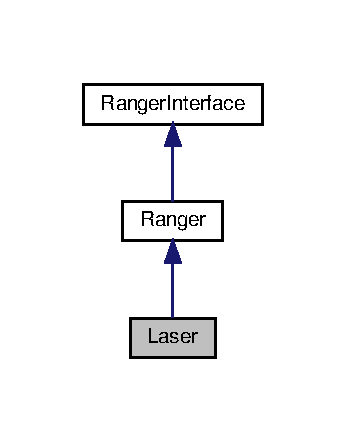
\includegraphics[width=166pt]{classLaser__inherit__graph}
\end{center}
\end{figure}


Collaboration diagram for Laser\+:\nopagebreak
\begin{figure}[H]
\begin{center}
\leavevmode
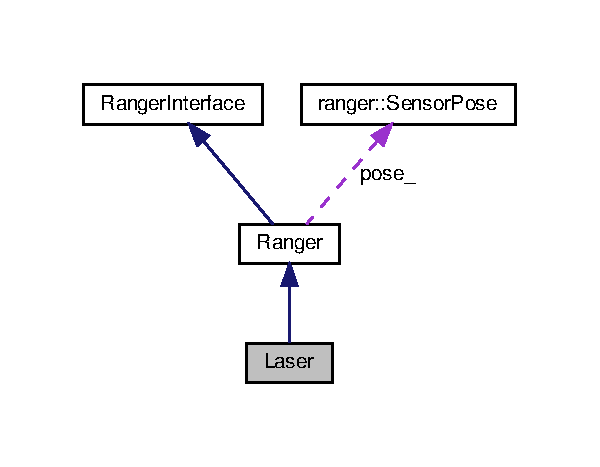
\includegraphics[width=288pt]{classLaser__coll__graph}
\end{center}
\end{figure}
\subsection*{Public Member Functions}
\begin{DoxyCompactItemize}
\item 
\mbox{\Hypertarget{classLaser_a5e1e9352d378edde419929165fa267d1}\label{classLaser_a5e1e9352d378edde419929165fa267d1}} 
void \hyperlink{classLaser_a5e1e9352d378edde419929165fa267d1}{get\+Set\+Params} (void)
\begin{DoxyCompactList}\small\item\em Prints out the parameters of the sensor that cannot be altered. \end{DoxyCompactList}\end{DoxyCompactItemize}
\subsection*{Additional Inherited Members}


The documentation for this class was generated from the following files\+:\begin{DoxyCompactItemize}
\item 
laser.\+h\item 
laser.\+cpp\end{DoxyCompactItemize}

\hypertarget{structgeometry__msgs_1_1Point}{}\section{geometry\+\_\+msgs\+:\+:Point Struct Reference}
\label{structgeometry__msgs_1_1Point}\index{geometry\+\_\+msgs\+::\+Point@{geometry\+\_\+msgs\+::\+Point}}


{\ttfamily \#include $<$analysis.\+h$>$}

\subsection*{Public Attributes}
\begin{DoxyCompactItemize}
\item 
\mbox{\Hypertarget{structgeometry__msgs_1_1Point_a52ccd2ddf703b661ed049c2a41e1525f}\label{structgeometry__msgs_1_1Point_a52ccd2ddf703b661ed049c2a41e1525f}} 
double {\bfseries x}
\item 
\mbox{\Hypertarget{structgeometry__msgs_1_1Point_a8b028e43156db47fed28583d9b196d89}\label{structgeometry__msgs_1_1Point_a8b028e43156db47fed28583d9b196d89}} 
double {\bfseries y}
\end{DoxyCompactItemize}


\subsection{Detailed Description}
Structure for 2d Positions 

The documentation for this struct was generated from the following file\+:\begin{DoxyCompactItemize}
\item 
\hyperlink{analysis_8h}{analysis.\+h}\end{DoxyCompactItemize}

\hypertarget{classRanger}{}\section{Ranger Class Reference}
\label{classRanger}\index{Ranger@{Ranger}}


Inheritance diagram for Ranger\+:\nopagebreak
\begin{figure}[H]
\begin{center}
\leavevmode
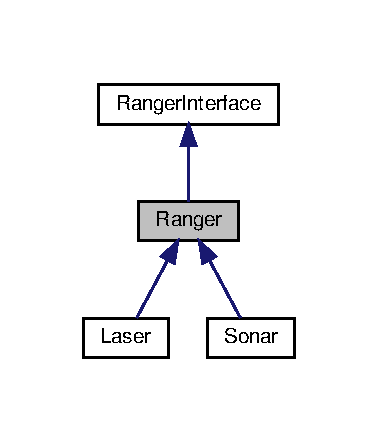
\includegraphics[width=182pt]{classRanger__inherit__graph}
\end{center}
\end{figure}


Collaboration diagram for Ranger\+:\nopagebreak
\begin{figure}[H]
\begin{center}
\leavevmode
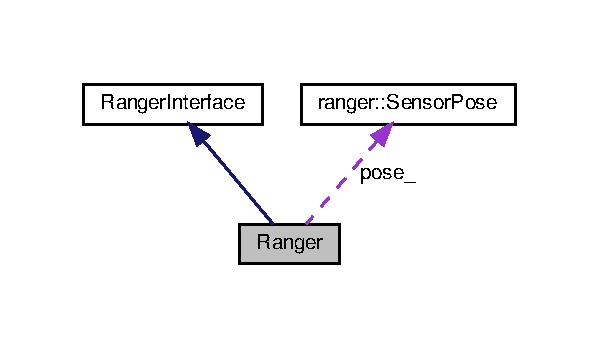
\includegraphics[width=288pt]{classRanger__coll__graph}
\end{center}
\end{figure}
\subsection*{Public Member Functions}
\begin{DoxyCompactItemize}
\item 
std\+::vector$<$ double $>$ \hyperlink{classRanger_a2b76dc3e21da8a7abac830d09fa81241}{generate\+Data} ()
\begin{DoxyCompactList}\small\item\em Randomly generates data for the sensor within its set parameters. \end{DoxyCompactList}\item 
unsigned int \hyperlink{classRanger_a95b5013ae191d1e19b93fab002306718}{get\+Angular\+Resolution} (void)
\item 
bool \hyperlink{classRanger_a3dc62dcba54eefbd7a0f08cbf97d87dc}{set\+Angular\+Resolution} (unsigned int resolution)
\item 
\hyperlink{structranger_1_1SensorPose}{ranger\+::\+Sensor\+Pose} \hyperlink{classRanger_aec1e730fbf4b46b01b08f6655152fc39}{get\+Sensor\+Pose} (void)
\item 
bool \hyperlink{classRanger_aa55ad45d83b8c095a495677ac8873f2b}{set\+Sensor\+Pose} (\hyperlink{structranger_1_1SensorPose}{ranger\+::\+Sensor\+Pose} pose)
\item 
unsigned int \hyperlink{classRanger_a4bca7dce56b7959257d90b1f30bf0271}{get\+Field\+Of\+View} (void)
\item 
bool \hyperlink{classRanger_afb5d392ca450bcce295e61c121d09157}{set\+Field\+Of\+View} (unsigned int fov)
\item 
double \hyperlink{classRanger_aba5e81260e55089d9ff869051156a722}{get\+Max\+Range} (void)
\item 
double \hyperlink{classRanger_a646a06d3916179b9ebc4502bad169eec}{get\+Min\+Range} (void)
\item 
\mbox{\Hypertarget{classRanger_a1f130ca82371febca9777a07f1a6a3e6}\label{classRanger_a1f130ca82371febca9777a07f1a6a3e6}} 
virtual void \hyperlink{classRanger_a1f130ca82371febca9777a07f1a6a3e6}{get\+Set\+Params} (void)
\begin{DoxyCompactList}\small\item\em Prints out the parameters of the sensor that cannot be altered. \end{DoxyCompactList}\item 
\hyperlink{namespaceranger_ab04465c229cc50595ffe40a891a3b135}{ranger\+::\+Sensing\+Method} \hyperlink{classRanger_a47e30b7ec55adec5bb542278ccfee140}{get\+Sensing\+Method} (void)
\item 
double \hyperlink{classRanger_a1cad662a106b1df8729846ea256f40c8}{get\+Sequence\+Number} (void)
\begin{DoxyCompactList}\small\item\em Get the Num Samples object or Sequence Number. \end{DoxyCompactList}\end{DoxyCompactItemize}
\subsection*{Protected Attributes}
\begin{DoxyCompactItemize}
\item 
\mbox{\Hypertarget{classRanger_a63dd9ac2ff81dc57ad9bf36d16f1da31}\label{classRanger_a63dd9ac2ff81dc57ad9bf36d16f1da31}} 
double {\bfseries maxrange\+\_\+}
\item 
\mbox{\Hypertarget{classRanger_a934b3e696fdb5ca2251eb4c9e7f8540d}\label{classRanger_a934b3e696fdb5ca2251eb4c9e7f8540d}} 
double {\bfseries minrange\+\_\+}
\item 
\mbox{\Hypertarget{classRanger_a013937201e2a4a516d4d36cac0193d68}\label{classRanger_a013937201e2a4a516d4d36cac0193d68}} 
unsigned int {\bfseries fov\+\_\+}
\item 
\mbox{\Hypertarget{classRanger_a92c38c7725afb93aa247b3d5ea3989ef}\label{classRanger_a92c38c7725afb93aa247b3d5ea3989ef}} 
\hyperlink{structranger_1_1SensorPose}{ranger\+::\+Sensor\+Pose} {\bfseries pose\+\_\+}
\item 
\mbox{\Hypertarget{classRanger_a9ccefbbcacf126ac6485ae26ff550092}\label{classRanger_a9ccefbbcacf126ac6485ae26ff550092}} 
unsigned int {\bfseries resolution\+\_\+}
\item 
\mbox{\Hypertarget{classRanger_a0fb0340a9d148fd0d1b63c600b81ec36}\label{classRanger_a0fb0340a9d148fd0d1b63c600b81ec36}} 
\hyperlink{namespaceranger_ab04465c229cc50595ffe40a891a3b135}{ranger\+::\+Sensing\+Method} {\bfseries method\+\_\+}
\item 
\mbox{\Hypertarget{classRanger_aada686d9a39d7899cd2dcae857c32ee4}\label{classRanger_aada686d9a39d7899cd2dcae857c32ee4}} 
std\+::string {\bfseries modelname\+\_\+}
\item 
\mbox{\Hypertarget{classRanger_a4912a54c69e4b2bf667e4b83f17414e3}\label{classRanger_a4912a54c69e4b2bf667e4b83f17414e3}} 
double {\bfseries num\+Readings\+\_\+}
\item 
\mbox{\Hypertarget{classRanger_a8b6dc0103ba424ff3c607d47b24077b8}\label{classRanger_a8b6dc0103ba424ff3c607d47b24077b8}} 
double {\bfseries num\+Samples\+\_\+}
\item 
\mbox{\Hypertarget{classRanger_a733a8974ad082a7bedacd346c0f42d26}\label{classRanger_a733a8974ad082a7bedacd346c0f42d26}} 
bool {\bfseries fov\+\_\+set\+\_\+}
\end{DoxyCompactItemize}


\subsection{Member Function Documentation}
\mbox{\Hypertarget{classRanger_a2b76dc3e21da8a7abac830d09fa81241}\label{classRanger_a2b76dc3e21da8a7abac830d09fa81241}} 
\index{Ranger@{Ranger}!generate\+Data@{generate\+Data}}
\index{generate\+Data@{generate\+Data}!Ranger@{Ranger}}
\subsubsection{\texorpdfstring{generate\+Data()}{generateData()}}
{\footnotesize\ttfamily std\+::vector$<$ double $>$ Ranger\+::generate\+Data (\begin{DoxyParamCaption}{ }\end{DoxyParamCaption})\hspace{0.3cm}{\ttfamily [virtual]}}



Randomly generates data for the sensor within its set parameters. 

\begin{DoxyReturn}{Returns}
std\+::vector$<$double$>$ 
\end{DoxyReturn}


Implements \hyperlink{classRangerInterface_a969c670cadf55a15733809116dc305c8}{Ranger\+Interface}.

\mbox{\Hypertarget{classRanger_a95b5013ae191d1e19b93fab002306718}\label{classRanger_a95b5013ae191d1e19b93fab002306718}} 
\index{Ranger@{Ranger}!get\+Angular\+Resolution@{get\+Angular\+Resolution}}
\index{get\+Angular\+Resolution@{get\+Angular\+Resolution}!Ranger@{Ranger}}
\subsubsection{\texorpdfstring{get\+Angular\+Resolution()}{getAngularResolution()}}
{\footnotesize\ttfamily unsigned int Ranger\+::get\+Angular\+Resolution (\begin{DoxyParamCaption}\item[{void}]{ }\end{DoxyParamCaption})\hspace{0.3cm}{\ttfamily [virtual]}}

Getter for Angular resolution \begin{DoxyReturn}{Returns}
angular resolution \mbox{[}deg\mbox{]} 
\end{DoxyReturn}


Implements \hyperlink{classRangerInterface_a37d4f89daffa8b2708dfc11034893552}{Ranger\+Interface}.

\mbox{\Hypertarget{classRanger_a4bca7dce56b7959257d90b1f30bf0271}\label{classRanger_a4bca7dce56b7959257d90b1f30bf0271}} 
\index{Ranger@{Ranger}!get\+Field\+Of\+View@{get\+Field\+Of\+View}}
\index{get\+Field\+Of\+View@{get\+Field\+Of\+View}!Ranger@{Ranger}}
\subsubsection{\texorpdfstring{get\+Field\+Of\+View()}{getFieldOfView()}}
{\footnotesize\ttfamily unsigned int Ranger\+::get\+Field\+Of\+View (\begin{DoxyParamCaption}\item[{void}]{ }\end{DoxyParamCaption})\hspace{0.3cm}{\ttfamily [virtual]}}

Getter for field of view, for P\+O\+I\+NT based sensors F\+OV is zero \begin{DoxyReturn}{Returns}
field of view \mbox{[}deg\mbox{]} 
\end{DoxyReturn}


Implements \hyperlink{classRangerInterface_a18716da6932402b8dda75f682be6f06c}{Ranger\+Interface}.

\mbox{\Hypertarget{classRanger_aba5e81260e55089d9ff869051156a722}\label{classRanger_aba5e81260e55089d9ff869051156a722}} 
\index{Ranger@{Ranger}!get\+Max\+Range@{get\+Max\+Range}}
\index{get\+Max\+Range@{get\+Max\+Range}!Ranger@{Ranger}}
\subsubsection{\texorpdfstring{get\+Max\+Range()}{getMaxRange()}}
{\footnotesize\ttfamily double Ranger\+::get\+Max\+Range (\begin{DoxyParamCaption}\item[{void}]{ }\end{DoxyParamCaption})\hspace{0.3cm}{\ttfamily [virtual]}}

Getter for maximum range \begin{DoxyReturn}{Returns}
maximum rage \mbox{[}m\mbox{]} 
\end{DoxyReturn}


Implements \hyperlink{classRangerInterface_a0bb29a41de5767c99081002c0590c186}{Ranger\+Interface}.

\mbox{\Hypertarget{classRanger_a646a06d3916179b9ebc4502bad169eec}\label{classRanger_a646a06d3916179b9ebc4502bad169eec}} 
\index{Ranger@{Ranger}!get\+Min\+Range@{get\+Min\+Range}}
\index{get\+Min\+Range@{get\+Min\+Range}!Ranger@{Ranger}}
\subsubsection{\texorpdfstring{get\+Min\+Range()}{getMinRange()}}
{\footnotesize\ttfamily double Ranger\+::get\+Min\+Range (\begin{DoxyParamCaption}\item[{void}]{ }\end{DoxyParamCaption})\hspace{0.3cm}{\ttfamily [virtual]}}

Getter for mimimum range \begin{DoxyReturn}{Returns}
minimum rage \mbox{[}m\mbox{]} 
\end{DoxyReturn}


Implements \hyperlink{classRangerInterface_ae6d501ddeeaad4a7b44d7d51ce64cb88}{Ranger\+Interface}.

\mbox{\Hypertarget{classRanger_a47e30b7ec55adec5bb542278ccfee140}\label{classRanger_a47e30b7ec55adec5bb542278ccfee140}} 
\index{Ranger@{Ranger}!get\+Sensing\+Method@{get\+Sensing\+Method}}
\index{get\+Sensing\+Method@{get\+Sensing\+Method}!Ranger@{Ranger}}
\subsubsection{\texorpdfstring{get\+Sensing\+Method()}{getSensingMethod()}}
{\footnotesize\ttfamily \hyperlink{namespaceranger_ab04465c229cc50595ffe40a891a3b135}{ranger\+::\+Sensing\+Method} Ranger\+::get\+Sensing\+Method (\begin{DoxyParamCaption}\item[{void}]{ }\end{DoxyParamCaption})\hspace{0.3cm}{\ttfamily [virtual]}}

Getter for sensing method \begin{DoxyReturn}{Returns}
Sensing Method 
\end{DoxyReturn}
\begin{DoxySeeAlso}{See also}
Sensging Method 
\end{DoxySeeAlso}


Implements \hyperlink{classRangerInterface_aeb06b9835f2b162b81917bd27797549b}{Ranger\+Interface}.

\mbox{\Hypertarget{classRanger_aec1e730fbf4b46b01b08f6655152fc39}\label{classRanger_aec1e730fbf4b46b01b08f6655152fc39}} 
\index{Ranger@{Ranger}!get\+Sensor\+Pose@{get\+Sensor\+Pose}}
\index{get\+Sensor\+Pose@{get\+Sensor\+Pose}!Ranger@{Ranger}}
\subsubsection{\texorpdfstring{get\+Sensor\+Pose()}{getSensorPose()}}
{\footnotesize\ttfamily \hyperlink{structranger_1_1SensorPose}{ranger\+::\+Sensor\+Pose} Ranger\+::get\+Sensor\+Pose (\begin{DoxyParamCaption}\item[{void}]{ }\end{DoxyParamCaption})\hspace{0.3cm}{\ttfamily [virtual]}}

Getter for sensor pose \begin{DoxyReturn}{Returns}
sensor pose 
\end{DoxyReturn}


Implements \hyperlink{classRangerInterface_a7f6db3f603d997ad6c5aa5c7778261f4}{Ranger\+Interface}.

\mbox{\Hypertarget{classRanger_a1cad662a106b1df8729846ea256f40c8}\label{classRanger_a1cad662a106b1df8729846ea256f40c8}} 
\index{Ranger@{Ranger}!get\+Sequence\+Number@{get\+Sequence\+Number}}
\index{get\+Sequence\+Number@{get\+Sequence\+Number}!Ranger@{Ranger}}
\subsubsection{\texorpdfstring{get\+Sequence\+Number()}{getSequenceNumber()}}
{\footnotesize\ttfamily double Ranger\+::get\+Sequence\+Number (\begin{DoxyParamCaption}\item[{void}]{ }\end{DoxyParamCaption})}



Get the Num Samples object or Sequence Number. 

\begin{DoxyReturn}{Returns}
double 
\end{DoxyReturn}
\mbox{\Hypertarget{classRanger_a3dc62dcba54eefbd7a0f08cbf97d87dc}\label{classRanger_a3dc62dcba54eefbd7a0f08cbf97d87dc}} 
\index{Ranger@{Ranger}!set\+Angular\+Resolution@{set\+Angular\+Resolution}}
\index{set\+Angular\+Resolution@{set\+Angular\+Resolution}!Ranger@{Ranger}}
\subsubsection{\texorpdfstring{set\+Angular\+Resolution()}{setAngularResolution()}}
{\footnotesize\ttfamily bool Ranger\+::set\+Angular\+Resolution (\begin{DoxyParamCaption}\item[{unsigned int}]{resolution }\end{DoxyParamCaption})\hspace{0.3cm}{\ttfamily [virtual]}}

Set angular resolution method 
\begin{DoxyParams}{Parameters}
{\em resolution} & in \mbox{[}degrees\mbox{]} \\
\hline
\end{DoxyParams}
\begin{DoxyReturn}{Returns}
true if resolution supported and actioned, false is not -\/ previous setting used 
\end{DoxyReturn}


Implements \hyperlink{classRangerInterface_aecffc9bbb58379da741c18326b9e41db}{Ranger\+Interface}.

\mbox{\Hypertarget{classRanger_afb5d392ca450bcce295e61c121d09157}\label{classRanger_afb5d392ca450bcce295e61c121d09157}} 
\index{Ranger@{Ranger}!set\+Field\+Of\+View@{set\+Field\+Of\+View}}
\index{set\+Field\+Of\+View@{set\+Field\+Of\+View}!Ranger@{Ranger}}
\subsubsection{\texorpdfstring{set\+Field\+Of\+View()}{setFieldOfView()}}
{\footnotesize\ttfamily bool Ranger\+::set\+Field\+Of\+View (\begin{DoxyParamCaption}\item[{unsigned int}]{fov }\end{DoxyParamCaption})\hspace{0.3cm}{\ttfamily [virtual]}}

Set field of view 
\begin{DoxyParams}{Parameters}
{\em field} & of view \mbox{[}degrees\mbox{]} \\
\hline
\end{DoxyParams}
\begin{DoxyReturn}{Returns}
true if field of view actioned, false otherwise 
\end{DoxyReturn}


Implements \hyperlink{classRangerInterface_a70357ca516198af45e2d503ef6af8f9f}{Ranger\+Interface}.

\mbox{\Hypertarget{classRanger_aa55ad45d83b8c095a495677ac8873f2b}\label{classRanger_aa55ad45d83b8c095a495677ac8873f2b}} 
\index{Ranger@{Ranger}!set\+Sensor\+Pose@{set\+Sensor\+Pose}}
\index{set\+Sensor\+Pose@{set\+Sensor\+Pose}!Ranger@{Ranger}}
\subsubsection{\texorpdfstring{set\+Sensor\+Pose()}{setSensorPose()}}
{\footnotesize\ttfamily bool Ranger\+::set\+Sensor\+Pose (\begin{DoxyParamCaption}\item[{\hyperlink{structranger_1_1SensorPose}{ranger\+::\+Sensor\+Pose}}]{pose }\end{DoxyParamCaption})\hspace{0.3cm}{\ttfamily [virtual]}}

Set sensor pose 
\begin{DoxyParams}{Parameters}
{\em pose} & Sensor\+Pose \\
\hline
\end{DoxyParams}
\begin{DoxyReturn}{Returns}
true if offset actioned, false otherwise 
\end{DoxyReturn}


Implements \hyperlink{classRangerInterface_a452301937b5ace7ded943d8aa76a061f}{Ranger\+Interface}.



The documentation for this class was generated from the following files\+:\begin{DoxyCompactItemize}
\item 
ranger.\+h\item 
ranger.\+cpp\end{DoxyCompactItemize}

\hypertarget{classRangerFusion}{}\section{Ranger\+Fusion Class Reference}
\label{classRangerFusion}\index{Ranger\+Fusion@{Ranger\+Fusion}}


Inheritance diagram for Ranger\+Fusion\+:\nopagebreak
\begin{figure}[H]
\begin{center}
\leavevmode
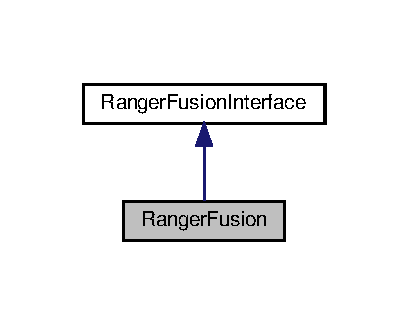
\includegraphics[width=196pt]{classRangerFusion__inherit__graph}
\end{center}
\end{figure}


Collaboration diagram for Ranger\+Fusion\+:\nopagebreak
\begin{figure}[H]
\begin{center}
\leavevmode
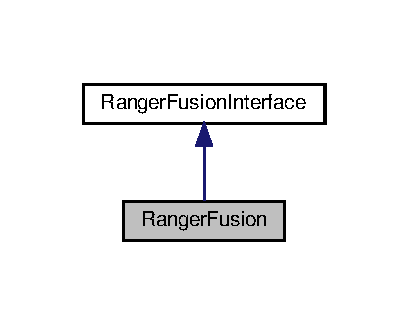
\includegraphics[width=196pt]{classRangerFusion__coll__graph}
\end{center}
\end{figure}
\subsection*{Public Member Functions}
\begin{DoxyCompactItemize}
\item 
\hyperlink{classRangerFusion_ae06d13fa52742f42e138b386e5022168}{Ranger\+Fusion} (std\+::vector$<$ \hyperlink{classRangerInterface}{Ranger\+Interface} $\ast$$>$ rangers)
\item 
void \hyperlink{classRangerFusion_a9b69869bd1e3bca155bcecbad5ea463b}{set\+Cells} (std\+::vector$<$ \hyperlink{classCell}{Cell} $\ast$$>$ cells)
\begin{DoxyCompactList}\small\item\em Accepts the container of cells. \end{DoxyCompactList}\item 
\mbox{\Hypertarget{classRangerFusion_aa9265f72bc3572567c9cf98cf6d9f0e1}\label{classRangerFusion_aa9265f72bc3572567c9cf98cf6d9f0e1}} 
void \hyperlink{classRangerFusion_aa9265f72bc3572567c9cf98cf6d9f0e1}{grab\+And\+Fuse\+Data} ()
\begin{DoxyCompactList}\small\item\em Does two operations (1) Calls each ranger to generate data and uses this data to determine colissions with provided container of cells (2) Generates a \textquotesingle{}fusion\textquotesingle{} of the data based on collision conditions as descibed in Assignment 2 specification. \end{DoxyCompactList}\item 
std\+::vector$<$ std\+::vector$<$ double $>$ $>$ \hyperlink{classRangerFusion_a5780383fdffe121a7a2372a047819ba9}{get\+Raw\+Range\+Data} ()
\begin{DoxyCompactList}\small\item\em Returns the raw data from all sensors in the ranger container within a vector of vectors The raw data is updated every time a new fusion is requested (grab\+And\+Fuse\+Dat). The raw data is the data used for collision checking. If no fusion has occured the vector shall be empty. N\+O\+TE\+: Cells positioned ON the sensor will be reported as U\+N\+K\+O\+WN. \end{DoxyCompactList}\item 
double \hyperlink{classRangerFusion_a7215e5405e808b5a853984e2b70ed6ad}{get\+Scanning\+Area} ()
\begin{DoxyCompactList}\small\item\em Returns the total scanning area possible with C\+O\+NE based scanners supplied A union of all areas \href{https://en.wikipedia.org/wiki/Union_(set_theory)}{\tt https\+://en.\+wikipedia.\+org/wiki/\+Union\+\_\+(set\+\_\+theory)} \end{DoxyCompactList}\end{DoxyCompactItemize}


\subsection{Constructor \& Destructor Documentation}
\mbox{\Hypertarget{classRangerFusion_ae06d13fa52742f42e138b386e5022168}\label{classRangerFusion_ae06d13fa52742f42e138b386e5022168}} 
\index{Ranger\+Fusion@{Ranger\+Fusion}!Ranger\+Fusion@{Ranger\+Fusion}}
\index{Ranger\+Fusion@{Ranger\+Fusion}!Ranger\+Fusion@{Ranger\+Fusion}}
\subsubsection{\texorpdfstring{Ranger\+Fusion()}{RangerFusion()}}
{\footnotesize\ttfamily Ranger\+Fusion\+::\+Ranger\+Fusion (\begin{DoxyParamCaption}\item[{std\+::vector$<$ \hyperlink{classRangerInterface}{Ranger\+Interface} $\ast$$>$}]{rangers }\end{DoxyParamCaption})}

The Default constructor sets the cell centre to values within the \#\+M\+A\+P\+\_\+\+S\+I\+ZE~\newline
\begin{DoxySeeAlso}{See also}
\hyperlink{classRangerFusionInterface}{Ranger\+Fusion\+Interface} and 

\hyperlink{classRangerInterface}{Ranger\+Interface} for more information 
\end{DoxySeeAlso}


\subsection{Member Function Documentation}
\mbox{\Hypertarget{classRangerFusion_a5780383fdffe121a7a2372a047819ba9}\label{classRangerFusion_a5780383fdffe121a7a2372a047819ba9}} 
\index{Ranger\+Fusion@{Ranger\+Fusion}!get\+Raw\+Range\+Data@{get\+Raw\+Range\+Data}}
\index{get\+Raw\+Range\+Data@{get\+Raw\+Range\+Data}!Ranger\+Fusion@{Ranger\+Fusion}}
\subsubsection{\texorpdfstring{get\+Raw\+Range\+Data()}{getRawRangeData()}}
{\footnotesize\ttfamily std\+::vector$<$ std\+::vector$<$ double $>$ $>$ Ranger\+Fusion\+::get\+Raw\+Range\+Data (\begin{DoxyParamCaption}{ }\end{DoxyParamCaption})\hspace{0.3cm}{\ttfamily [virtual]}}



Returns the raw data from all sensors in the ranger container within a vector of vectors The raw data is updated every time a new fusion is requested (grab\+And\+Fuse\+Dat). The raw data is the data used for collision checking. If no fusion has occured the vector shall be empty. N\+O\+TE\+: Cells positioned ON the sensor will be reported as U\+N\+K\+O\+WN. 

\begin{DoxyReturn}{Returns}
std\+::vector$<$std\+::vector$<$double$>$$>$ the outer elements of the vector related to the rangers, the inner elements of vector are the respective range readings
\end{DoxyReturn}
\begin{DoxySeeAlso}{See also}
\hyperlink{classRangerFusion_aa9265f72bc3572567c9cf98cf6d9f0e1}{grab\+And\+Fuse\+Data} 
\end{DoxySeeAlso}


Implements \hyperlink{classRangerFusionInterface_a9d60ca5866261026b870d7c0171587f5}{Ranger\+Fusion\+Interface}.

\mbox{\Hypertarget{classRangerFusion_a7215e5405e808b5a853984e2b70ed6ad}\label{classRangerFusion_a7215e5405e808b5a853984e2b70ed6ad}} 
\index{Ranger\+Fusion@{Ranger\+Fusion}!get\+Scanning\+Area@{get\+Scanning\+Area}}
\index{get\+Scanning\+Area@{get\+Scanning\+Area}!Ranger\+Fusion@{Ranger\+Fusion}}
\subsubsection{\texorpdfstring{get\+Scanning\+Area()}{getScanningArea()}}
{\footnotesize\ttfamily double Ranger\+Fusion\+::get\+Scanning\+Area (\begin{DoxyParamCaption}{ }\end{DoxyParamCaption})\hspace{0.3cm}{\ttfamily [virtual]}}



Returns the total scanning area possible with C\+O\+NE based scanners supplied A union of all areas \href{https://en.wikipedia.org/wiki/Union_(set_theory)}{\tt https\+://en.\+wikipedia.\+org/wiki/\+Union\+\_\+(set\+\_\+theory)} 

\begin{DoxyReturn}{Returns}
double Total area coverage
\end{DoxyReturn}
\begin{DoxySeeAlso}{See also}
\hyperlink{classRangerFusion_aa9265f72bc3572567c9cf98cf6d9f0e1}{grab\+And\+Fuse\+Data} 
\end{DoxySeeAlso}


Implements \hyperlink{classRangerFusionInterface_a65155605804376da4f67baf3c6f97f40}{Ranger\+Fusion\+Interface}.

\mbox{\Hypertarget{classRangerFusion_a9b69869bd1e3bca155bcecbad5ea463b}\label{classRangerFusion_a9b69869bd1e3bca155bcecbad5ea463b}} 
\index{Ranger\+Fusion@{Ranger\+Fusion}!set\+Cells@{set\+Cells}}
\index{set\+Cells@{set\+Cells}!Ranger\+Fusion@{Ranger\+Fusion}}
\subsubsection{\texorpdfstring{set\+Cells()}{setCells()}}
{\footnotesize\ttfamily void Ranger\+Fusion\+::set\+Cells (\begin{DoxyParamCaption}\item[{std\+::vector$<$ \hyperlink{classCell}{Cell} $\ast$$>$}]{cells }\end{DoxyParamCaption})\hspace{0.3cm}{\ttfamily [virtual]}}



Accepts the container of cells. 


\begin{DoxyParams}{Parameters}
{\em cells} & \\
\hline
\end{DoxyParams}


Implements \hyperlink{classRangerFusionInterface_ab8fdee0050521767d33179a63da91e4f}{Ranger\+Fusion\+Interface}.



The documentation for this class was generated from the following files\+:\begin{DoxyCompactItemize}
\item 
rangerfusion.\+h\item 
rangerfusion.\+cpp\end{DoxyCompactItemize}

\hypertarget{classRangerFusionInterface}{}\section{Ranger\+Fusion\+Interface Class Reference}
\label{classRangerFusionInterface}\index{Ranger\+Fusion\+Interface@{Ranger\+Fusion\+Interface}}


Specifies the required interface for your \hyperlink{classRangerFusion}{Ranger\+Fusion} class your ranger fusion class must inherit from it. {\bfseries  You M\+U\+ST N\+OT edit this file }.  




{\ttfamily \#include $<$rangerfusioninterface.\+h$>$}



Inheritance diagram for Ranger\+Fusion\+Interface\+:\nopagebreak
\begin{figure}[H]
\begin{center}
\leavevmode
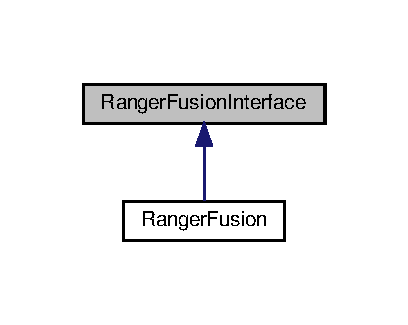
\includegraphics[width=196pt]{classRangerFusionInterface__inherit__graph}
\end{center}
\end{figure}
\subsection*{Public Member Functions}
\begin{DoxyCompactItemize}
\item 
virtual void \hyperlink{classRangerFusionInterface_ab8fdee0050521767d33179a63da91e4f}{set\+Cells} (std\+::vector$<$ \hyperlink{classCell}{Cell} $\ast$$>$ cells)=0
\begin{DoxyCompactList}\small\item\em Accepts the container of cells. \end{DoxyCompactList}\item 
\mbox{\Hypertarget{classRangerFusionInterface_ada6afdab2ce6d58a1bd0134f5e2be23f}\label{classRangerFusionInterface_ada6afdab2ce6d58a1bd0134f5e2be23f}} 
virtual void \hyperlink{classRangerFusionInterface_ada6afdab2ce6d58a1bd0134f5e2be23f}{grab\+And\+Fuse\+Data} ()=0
\begin{DoxyCompactList}\small\item\em Does two operations (1) Calls each ranger to generate data and uses this data to determine colissions with provided container of cells (2) Generates a \textquotesingle{}fusion\textquotesingle{} of the data based on collision conditions as descibed in Assignment 2 specification. \end{DoxyCompactList}\item 
virtual std\+::vector$<$ std\+::vector$<$ double $>$ $>$ \hyperlink{classRangerFusionInterface_a9d60ca5866261026b870d7c0171587f5}{get\+Raw\+Range\+Data} ()=0
\begin{DoxyCompactList}\small\item\em Returns the raw data from all sensors in the ranger container within a vector of vectors The raw data is updated every time a new fusion is requested (grab\+And\+Fuse\+Dat). The raw data is the data used for collision checking. If no fusion has occured the vector shall be empty. N\+O\+TE\+: Cells positioned ON the sensor will be reported as U\+N\+K\+O\+WN. \end{DoxyCompactList}\item 
virtual double \hyperlink{classRangerFusionInterface_a65155605804376da4f67baf3c6f97f40}{get\+Scanning\+Area} ()=0
\begin{DoxyCompactList}\small\item\em Returns the total scanning area possible with C\+O\+NE based scanners supplied A union of all areas \href{https://en.wikipedia.org/wiki/Union_(set_theory)}{\tt https\+://en.\+wikipedia.\+org/wiki/\+Union\+\_\+(set\+\_\+theory)} \end{DoxyCompactList}\end{DoxyCompactItemize}


\subsection{Detailed Description}
Specifies the required interface for your \hyperlink{classRangerFusion}{Ranger\+Fusion} class your ranger fusion class must inherit from it. {\bfseries  You M\+U\+ST N\+OT edit this file }. 

\hyperlink{classRanger}{Ranger} Interface Class

Specifies the required interface for your \hyperlink{classRangerFusion}{Ranger\+Fusion} class your ranger fusion class must inherit from it. {\bfseries  You M\+U\+ST N\+OT edit this file }. \begin{DoxyAuthor}{Author}
Alen Alempijevic 
\end{DoxyAuthor}
\begin{DoxyVersion}{Version}
1.\+01-\/2 
\end{DoxyVersion}
\begin{DoxyDate}{Date}
2019-\/07-\/10 
\end{DoxyDate}
\begin{DoxyPrecond}{Precondition}
none 
\end{DoxyPrecond}
\begin{DoxyRefDesc}{Bug}
\item[\hyperlink{bug__bug000002}{Bug}]none reported as of 2020-\/04-\/11 \end{DoxyRefDesc}
\begin{DoxyWarning}{Warning}
students M\+U\+ST N\+OT change this class (the header file) 
\end{DoxyWarning}


\subsection{Member Function Documentation}
\mbox{\Hypertarget{classRangerFusionInterface_a9d60ca5866261026b870d7c0171587f5}\label{classRangerFusionInterface_a9d60ca5866261026b870d7c0171587f5}} 
\index{Ranger\+Fusion\+Interface@{Ranger\+Fusion\+Interface}!get\+Raw\+Range\+Data@{get\+Raw\+Range\+Data}}
\index{get\+Raw\+Range\+Data@{get\+Raw\+Range\+Data}!Ranger\+Fusion\+Interface@{Ranger\+Fusion\+Interface}}
\subsubsection{\texorpdfstring{get\+Raw\+Range\+Data()}{getRawRangeData()}}
{\footnotesize\ttfamily virtual std\+::vector$<$std\+::vector$<$double$>$ $>$ Ranger\+Fusion\+Interface\+::get\+Raw\+Range\+Data (\begin{DoxyParamCaption}{ }\end{DoxyParamCaption})\hspace{0.3cm}{\ttfamily [pure virtual]}}



Returns the raw data from all sensors in the ranger container within a vector of vectors The raw data is updated every time a new fusion is requested (grab\+And\+Fuse\+Dat). The raw data is the data used for collision checking. If no fusion has occured the vector shall be empty. N\+O\+TE\+: Cells positioned ON the sensor will be reported as U\+N\+K\+O\+WN. 

\begin{DoxyReturn}{Returns}
std\+::vector$<$std\+::vector$<$double$>$$>$ the outer elements of the vector related to the rangers, the inner elements of vector are the respective range readings
\end{DoxyReturn}
\begin{DoxySeeAlso}{See also}
\hyperlink{classRangerFusionInterface_ada6afdab2ce6d58a1bd0134f5e2be23f}{grab\+And\+Fuse\+Data} 
\end{DoxySeeAlso}


Implemented in \hyperlink{classRangerFusion_a5780383fdffe121a7a2372a047819ba9}{Ranger\+Fusion}.

\mbox{\Hypertarget{classRangerFusionInterface_a65155605804376da4f67baf3c6f97f40}\label{classRangerFusionInterface_a65155605804376da4f67baf3c6f97f40}} 
\index{Ranger\+Fusion\+Interface@{Ranger\+Fusion\+Interface}!get\+Scanning\+Area@{get\+Scanning\+Area}}
\index{get\+Scanning\+Area@{get\+Scanning\+Area}!Ranger\+Fusion\+Interface@{Ranger\+Fusion\+Interface}}
\subsubsection{\texorpdfstring{get\+Scanning\+Area()}{getScanningArea()}}
{\footnotesize\ttfamily virtual double Ranger\+Fusion\+Interface\+::get\+Scanning\+Area (\begin{DoxyParamCaption}{ }\end{DoxyParamCaption})\hspace{0.3cm}{\ttfamily [pure virtual]}}



Returns the total scanning area possible with C\+O\+NE based scanners supplied A union of all areas \href{https://en.wikipedia.org/wiki/Union_(set_theory)}{\tt https\+://en.\+wikipedia.\+org/wiki/\+Union\+\_\+(set\+\_\+theory)} 

\begin{DoxyReturn}{Returns}
double Total area coverage
\end{DoxyReturn}
\begin{DoxySeeAlso}{See also}
\hyperlink{classRangerFusionInterface_ada6afdab2ce6d58a1bd0134f5e2be23f}{grab\+And\+Fuse\+Data} 
\end{DoxySeeAlso}


Implemented in \hyperlink{classRangerFusion_a7215e5405e808b5a853984e2b70ed6ad}{Ranger\+Fusion}.

\mbox{\Hypertarget{classRangerFusionInterface_ab8fdee0050521767d33179a63da91e4f}\label{classRangerFusionInterface_ab8fdee0050521767d33179a63da91e4f}} 
\index{Ranger\+Fusion\+Interface@{Ranger\+Fusion\+Interface}!set\+Cells@{set\+Cells}}
\index{set\+Cells@{set\+Cells}!Ranger\+Fusion\+Interface@{Ranger\+Fusion\+Interface}}
\subsubsection{\texorpdfstring{set\+Cells()}{setCells()}}
{\footnotesize\ttfamily virtual void Ranger\+Fusion\+Interface\+::set\+Cells (\begin{DoxyParamCaption}\item[{std\+::vector$<$ \hyperlink{classCell}{Cell} $\ast$$>$}]{cells }\end{DoxyParamCaption})\hspace{0.3cm}{\ttfamily [pure virtual]}}



Accepts the container of cells. 


\begin{DoxyParams}{Parameters}
{\em cells} & \\
\hline
\end{DoxyParams}


Implemented in \hyperlink{classRangerFusion_a9b69869bd1e3bca155bcecbad5ea463b}{Ranger\+Fusion}.



The documentation for this class was generated from the following file\+:\begin{DoxyCompactItemize}
\item 
rangerfusioninterface.\+h\end{DoxyCompactItemize}

\hypertarget{classRangerInterface}{}\section{Ranger\+Interface Class Reference}
\label{classRangerInterface}\index{Ranger\+Interface@{Ranger\+Interface}}


Specifies the functionality for the \hyperlink{classRanger}{Ranger} Class, your \hyperlink{classRanger}{Ranger} class must inherit from it. {\bfseries  You M\+U\+ST N\+OT edit this file }.  




{\ttfamily \#include $<$rangerinterface.\+h$>$}



Inheritance diagram for Ranger\+Interface\+:\nopagebreak
\begin{figure}[H]
\begin{center}
\leavevmode
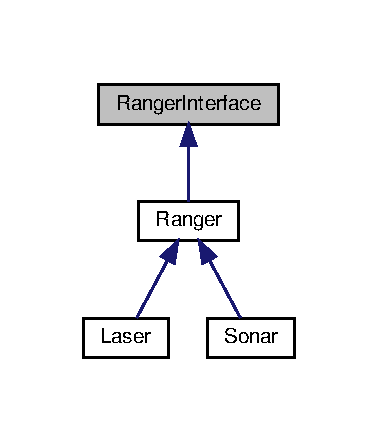
\includegraphics[width=182pt]{classRangerInterface__inherit__graph}
\end{center}
\end{figure}
\subsection*{Public Member Functions}
\begin{DoxyCompactItemize}
\item 
virtual std\+::vector$<$ double $>$ \hyperlink{classRangerInterface_a969c670cadf55a15733809116dc305c8}{generate\+Data} ()=0
\begin{DoxyCompactList}\small\item\em Randomly generates data for the sensor within its set parameters. \end{DoxyCompactList}\item 
virtual unsigned int \hyperlink{classRangerInterface_a37d4f89daffa8b2708dfc11034893552}{get\+Angular\+Resolution} (void)=0
\item 
virtual \hyperlink{structranger_1_1SensorPose}{ranger\+::\+Sensor\+Pose} \hyperlink{classRangerInterface_a7f6db3f603d997ad6c5aa5c7778261f4}{get\+Sensor\+Pose} (void)=0
\item 
virtual unsigned int \hyperlink{classRangerInterface_a18716da6932402b8dda75f682be6f06c}{get\+Field\+Of\+View} (void)=0
\item 
virtual double \hyperlink{classRangerInterface_a0bb29a41de5767c99081002c0590c186}{get\+Max\+Range} (void)=0
\item 
virtual double \hyperlink{classRangerInterface_ae6d501ddeeaad4a7b44d7d51ce64cb88}{get\+Min\+Range} (void)=0
\item 
virtual \hyperlink{namespaceranger_ab04465c229cc50595ffe40a891a3b135}{ranger\+::\+Sensing\+Method} \hyperlink{classRangerInterface_aeb06b9835f2b162b81917bd27797549b}{get\+Sensing\+Method} (void)=0
\item 
virtual bool \hyperlink{classRangerInterface_aecffc9bbb58379da741c18326b9e41db}{set\+Angular\+Resolution} (unsigned int resolution)=0
\item 
virtual bool \hyperlink{classRangerInterface_a452301937b5ace7ded943d8aa76a061f}{set\+Sensor\+Pose} (\hyperlink{structranger_1_1SensorPose}{ranger\+::\+Sensor\+Pose} pose)=0
\item 
virtual bool \hyperlink{classRangerInterface_a70357ca516198af45e2d503ef6af8f9f}{set\+Field\+Of\+View} (unsigned int fov)=0
\end{DoxyCompactItemize}


\subsection{Detailed Description}
Specifies the functionality for the \hyperlink{classRanger}{Ranger} Class, your \hyperlink{classRanger}{Ranger} class must inherit from it. {\bfseries  You M\+U\+ST N\+OT edit this file }. 

\subsection{Member Function Documentation}
\mbox{\Hypertarget{classRangerInterface_a969c670cadf55a15733809116dc305c8}\label{classRangerInterface_a969c670cadf55a15733809116dc305c8}} 
\index{Ranger\+Interface@{Ranger\+Interface}!generate\+Data@{generate\+Data}}
\index{generate\+Data@{generate\+Data}!Ranger\+Interface@{Ranger\+Interface}}
\subsubsection{\texorpdfstring{generate\+Data()}{generateData()}}
{\footnotesize\ttfamily virtual std\+::vector$<$double$>$ Ranger\+Interface\+::generate\+Data (\begin{DoxyParamCaption}{ }\end{DoxyParamCaption})\hspace{0.3cm}{\ttfamily [pure virtual]}}



Randomly generates data for the sensor within its set parameters. 

\begin{DoxyReturn}{Returns}
std\+::vector$<$double$>$ 
\end{DoxyReturn}


Implemented in \hyperlink{classRanger_a2b76dc3e21da8a7abac830d09fa81241}{Ranger}.

\mbox{\Hypertarget{classRangerInterface_a37d4f89daffa8b2708dfc11034893552}\label{classRangerInterface_a37d4f89daffa8b2708dfc11034893552}} 
\index{Ranger\+Interface@{Ranger\+Interface}!get\+Angular\+Resolution@{get\+Angular\+Resolution}}
\index{get\+Angular\+Resolution@{get\+Angular\+Resolution}!Ranger\+Interface@{Ranger\+Interface}}
\subsubsection{\texorpdfstring{get\+Angular\+Resolution()}{getAngularResolution()}}
{\footnotesize\ttfamily virtual unsigned int Ranger\+Interface\+::get\+Angular\+Resolution (\begin{DoxyParamCaption}\item[{void}]{ }\end{DoxyParamCaption})\hspace{0.3cm}{\ttfamily [pure virtual]}}

Getter for Angular resolution \begin{DoxyReturn}{Returns}
angular resolution \mbox{[}deg\mbox{]} 
\end{DoxyReturn}


Implemented in \hyperlink{classRanger_a95b5013ae191d1e19b93fab002306718}{Ranger}.

\mbox{\Hypertarget{classRangerInterface_a18716da6932402b8dda75f682be6f06c}\label{classRangerInterface_a18716da6932402b8dda75f682be6f06c}} 
\index{Ranger\+Interface@{Ranger\+Interface}!get\+Field\+Of\+View@{get\+Field\+Of\+View}}
\index{get\+Field\+Of\+View@{get\+Field\+Of\+View}!Ranger\+Interface@{Ranger\+Interface}}
\subsubsection{\texorpdfstring{get\+Field\+Of\+View()}{getFieldOfView()}}
{\footnotesize\ttfamily virtual unsigned int Ranger\+Interface\+::get\+Field\+Of\+View (\begin{DoxyParamCaption}\item[{void}]{ }\end{DoxyParamCaption})\hspace{0.3cm}{\ttfamily [pure virtual]}}

Getter for field of view, for P\+O\+I\+NT based sensors F\+OV is zero \begin{DoxyReturn}{Returns}
field of view \mbox{[}deg\mbox{]} 
\end{DoxyReturn}


Implemented in \hyperlink{classRanger_a4bca7dce56b7959257d90b1f30bf0271}{Ranger}.

\mbox{\Hypertarget{classRangerInterface_a0bb29a41de5767c99081002c0590c186}\label{classRangerInterface_a0bb29a41de5767c99081002c0590c186}} 
\index{Ranger\+Interface@{Ranger\+Interface}!get\+Max\+Range@{get\+Max\+Range}}
\index{get\+Max\+Range@{get\+Max\+Range}!Ranger\+Interface@{Ranger\+Interface}}
\subsubsection{\texorpdfstring{get\+Max\+Range()}{getMaxRange()}}
{\footnotesize\ttfamily virtual double Ranger\+Interface\+::get\+Max\+Range (\begin{DoxyParamCaption}\item[{void}]{ }\end{DoxyParamCaption})\hspace{0.3cm}{\ttfamily [pure virtual]}}

Getter for maximum range \begin{DoxyReturn}{Returns}
maximum rage \mbox{[}m\mbox{]} 
\end{DoxyReturn}


Implemented in \hyperlink{classRanger_aba5e81260e55089d9ff869051156a722}{Ranger}.

\mbox{\Hypertarget{classRangerInterface_ae6d501ddeeaad4a7b44d7d51ce64cb88}\label{classRangerInterface_ae6d501ddeeaad4a7b44d7d51ce64cb88}} 
\index{Ranger\+Interface@{Ranger\+Interface}!get\+Min\+Range@{get\+Min\+Range}}
\index{get\+Min\+Range@{get\+Min\+Range}!Ranger\+Interface@{Ranger\+Interface}}
\subsubsection{\texorpdfstring{get\+Min\+Range()}{getMinRange()}}
{\footnotesize\ttfamily virtual double Ranger\+Interface\+::get\+Min\+Range (\begin{DoxyParamCaption}\item[{void}]{ }\end{DoxyParamCaption})\hspace{0.3cm}{\ttfamily [pure virtual]}}

Getter for mimimum range \begin{DoxyReturn}{Returns}
minimum rage \mbox{[}m\mbox{]} 
\end{DoxyReturn}


Implemented in \hyperlink{classRanger_a646a06d3916179b9ebc4502bad169eec}{Ranger}.

\mbox{\Hypertarget{classRangerInterface_aeb06b9835f2b162b81917bd27797549b}\label{classRangerInterface_aeb06b9835f2b162b81917bd27797549b}} 
\index{Ranger\+Interface@{Ranger\+Interface}!get\+Sensing\+Method@{get\+Sensing\+Method}}
\index{get\+Sensing\+Method@{get\+Sensing\+Method}!Ranger\+Interface@{Ranger\+Interface}}
\subsubsection{\texorpdfstring{get\+Sensing\+Method()}{getSensingMethod()}}
{\footnotesize\ttfamily virtual \hyperlink{namespaceranger_ab04465c229cc50595ffe40a891a3b135}{ranger\+::\+Sensing\+Method} Ranger\+Interface\+::get\+Sensing\+Method (\begin{DoxyParamCaption}\item[{void}]{ }\end{DoxyParamCaption})\hspace{0.3cm}{\ttfamily [pure virtual]}}

Getter for sensing method \begin{DoxyReturn}{Returns}
Sensing Method 
\end{DoxyReturn}
\begin{DoxySeeAlso}{See also}
Sensging Method 
\end{DoxySeeAlso}


Implemented in \hyperlink{classRanger_a47e30b7ec55adec5bb542278ccfee140}{Ranger}.

\mbox{\Hypertarget{classRangerInterface_a7f6db3f603d997ad6c5aa5c7778261f4}\label{classRangerInterface_a7f6db3f603d997ad6c5aa5c7778261f4}} 
\index{Ranger\+Interface@{Ranger\+Interface}!get\+Sensor\+Pose@{get\+Sensor\+Pose}}
\index{get\+Sensor\+Pose@{get\+Sensor\+Pose}!Ranger\+Interface@{Ranger\+Interface}}
\subsubsection{\texorpdfstring{get\+Sensor\+Pose()}{getSensorPose()}}
{\footnotesize\ttfamily virtual \hyperlink{structranger_1_1SensorPose}{ranger\+::\+Sensor\+Pose} Ranger\+Interface\+::get\+Sensor\+Pose (\begin{DoxyParamCaption}\item[{void}]{ }\end{DoxyParamCaption})\hspace{0.3cm}{\ttfamily [pure virtual]}}

Getter for sensor pose \begin{DoxyReturn}{Returns}
sensor pose 
\end{DoxyReturn}


Implemented in \hyperlink{classRanger_aec1e730fbf4b46b01b08f6655152fc39}{Ranger}.

\mbox{\Hypertarget{classRangerInterface_aecffc9bbb58379da741c18326b9e41db}\label{classRangerInterface_aecffc9bbb58379da741c18326b9e41db}} 
\index{Ranger\+Interface@{Ranger\+Interface}!set\+Angular\+Resolution@{set\+Angular\+Resolution}}
\index{set\+Angular\+Resolution@{set\+Angular\+Resolution}!Ranger\+Interface@{Ranger\+Interface}}
\subsubsection{\texorpdfstring{set\+Angular\+Resolution()}{setAngularResolution()}}
{\footnotesize\ttfamily virtual bool Ranger\+Interface\+::set\+Angular\+Resolution (\begin{DoxyParamCaption}\item[{unsigned int}]{resolution }\end{DoxyParamCaption})\hspace{0.3cm}{\ttfamily [pure virtual]}}

Set angular resolution method 
\begin{DoxyParams}{Parameters}
{\em resolution} & in \mbox{[}degrees\mbox{]} \\
\hline
\end{DoxyParams}
\begin{DoxyReturn}{Returns}
true if resolution supported and actioned, false is not -\/ previous setting used 
\end{DoxyReturn}


Implemented in \hyperlink{classRanger_a3dc62dcba54eefbd7a0f08cbf97d87dc}{Ranger}.

\mbox{\Hypertarget{classRangerInterface_a70357ca516198af45e2d503ef6af8f9f}\label{classRangerInterface_a70357ca516198af45e2d503ef6af8f9f}} 
\index{Ranger\+Interface@{Ranger\+Interface}!set\+Field\+Of\+View@{set\+Field\+Of\+View}}
\index{set\+Field\+Of\+View@{set\+Field\+Of\+View}!Ranger\+Interface@{Ranger\+Interface}}
\subsubsection{\texorpdfstring{set\+Field\+Of\+View()}{setFieldOfView()}}
{\footnotesize\ttfamily virtual bool Ranger\+Interface\+::set\+Field\+Of\+View (\begin{DoxyParamCaption}\item[{unsigned int}]{fov }\end{DoxyParamCaption})\hspace{0.3cm}{\ttfamily [pure virtual]}}

Set field of view 
\begin{DoxyParams}{Parameters}
{\em field} & of view \mbox{[}degrees\mbox{]} \\
\hline
\end{DoxyParams}
\begin{DoxyReturn}{Returns}
true if field of view actioned, false otherwise 
\end{DoxyReturn}


Implemented in \hyperlink{classRanger_afb5d392ca450bcce295e61c121d09157}{Ranger}.

\mbox{\Hypertarget{classRangerInterface_a452301937b5ace7ded943d8aa76a061f}\label{classRangerInterface_a452301937b5ace7ded943d8aa76a061f}} 
\index{Ranger\+Interface@{Ranger\+Interface}!set\+Sensor\+Pose@{set\+Sensor\+Pose}}
\index{set\+Sensor\+Pose@{set\+Sensor\+Pose}!Ranger\+Interface@{Ranger\+Interface}}
\subsubsection{\texorpdfstring{set\+Sensor\+Pose()}{setSensorPose()}}
{\footnotesize\ttfamily virtual bool Ranger\+Interface\+::set\+Sensor\+Pose (\begin{DoxyParamCaption}\item[{\hyperlink{structranger_1_1SensorPose}{ranger\+::\+Sensor\+Pose}}]{pose }\end{DoxyParamCaption})\hspace{0.3cm}{\ttfamily [pure virtual]}}

Set sensor pose 
\begin{DoxyParams}{Parameters}
{\em pose} & Sensor\+Pose \\
\hline
\end{DoxyParams}
\begin{DoxyReturn}{Returns}
true if offset actioned, false otherwise 
\end{DoxyReturn}


Implemented in \hyperlink{classRanger_aa55ad45d83b8c095a495677ac8873f2b}{Ranger}.



The documentation for this class was generated from the following file\+:\begin{DoxyCompactItemize}
\item 
rangerinterface.\+h\end{DoxyCompactItemize}

\hypertarget{structranger_1_1SensorPose}{}\section{ranger\+:\+:Sensor\+Pose Struct Reference}
\label{structranger_1_1SensorPose}\index{ranger\+::\+Sensor\+Pose@{ranger\+::\+Sensor\+Pose}}
\subsection*{Public Attributes}
\begin{DoxyCompactItemize}
\item 
double \hyperlink{structranger_1_1SensorPose_af3f4cc40667c93d56dd8e672c38a75e1}{x}
\item 
double \hyperlink{structranger_1_1SensorPose_ae7a4c48860c2e9f4fe7de03f8008026f}{y}
\item 
double \hyperlink{structranger_1_1SensorPose_a18751d4e746969c536714b372e3df1f6}{theta}
\end{DoxyCompactItemize}


\subsection{Member Data Documentation}
\mbox{\Hypertarget{structranger_1_1SensorPose_a18751d4e746969c536714b372e3df1f6}\label{structranger_1_1SensorPose_a18751d4e746969c536714b372e3df1f6}} 
\index{ranger\+::\+Sensor\+Pose@{ranger\+::\+Sensor\+Pose}!theta@{theta}}
\index{theta@{theta}!ranger\+::\+Sensor\+Pose@{ranger\+::\+Sensor\+Pose}}
\subsubsection{\texorpdfstring{theta}{theta}}
{\footnotesize\ttfamily double ranger\+::\+Sensor\+Pose\+::theta}

sensor angle \mbox{[}radians\mbox{]} \mbox{\Hypertarget{structranger_1_1SensorPose_af3f4cc40667c93d56dd8e672c38a75e1}\label{structranger_1_1SensorPose_af3f4cc40667c93d56dd8e672c38a75e1}} 
\index{ranger\+::\+Sensor\+Pose@{ranger\+::\+Sensor\+Pose}!x@{x}}
\index{x@{x}!ranger\+::\+Sensor\+Pose@{ranger\+::\+Sensor\+Pose}}
\subsubsection{\texorpdfstring{x}{x}}
{\footnotesize\ttfamily double ranger\+::\+Sensor\+Pose\+::x}

sensor position x axis \mbox{[}m\mbox{]} \mbox{\Hypertarget{structranger_1_1SensorPose_ae7a4c48860c2e9f4fe7de03f8008026f}\label{structranger_1_1SensorPose_ae7a4c48860c2e9f4fe7de03f8008026f}} 
\index{ranger\+::\+Sensor\+Pose@{ranger\+::\+Sensor\+Pose}!y@{y}}
\index{y@{y}!ranger\+::\+Sensor\+Pose@{ranger\+::\+Sensor\+Pose}}
\subsubsection{\texorpdfstring{y}{y}}
{\footnotesize\ttfamily double ranger\+::\+Sensor\+Pose\+::y}

sensor position y axis \mbox{[}m\mbox{]} 

The documentation for this struct was generated from the following file\+:\begin{DoxyCompactItemize}
\item 
rangerinterface.\+h\end{DoxyCompactItemize}

\hypertarget{classSonar}{}\section{Sonar Class Reference}
\label{classSonar}\index{Sonar@{Sonar}}


Inheritance diagram for Sonar\+:\nopagebreak
\begin{figure}[H]
\begin{center}
\leavevmode
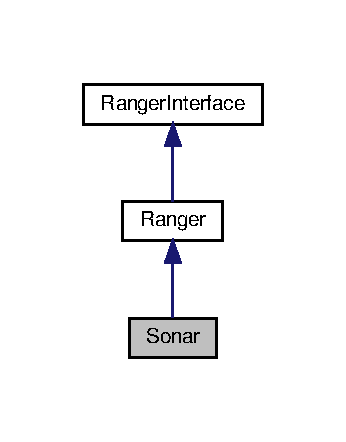
\includegraphics[width=166pt]{classSonar__inherit__graph}
\end{center}
\end{figure}


Collaboration diagram for Sonar\+:\nopagebreak
\begin{figure}[H]
\begin{center}
\leavevmode
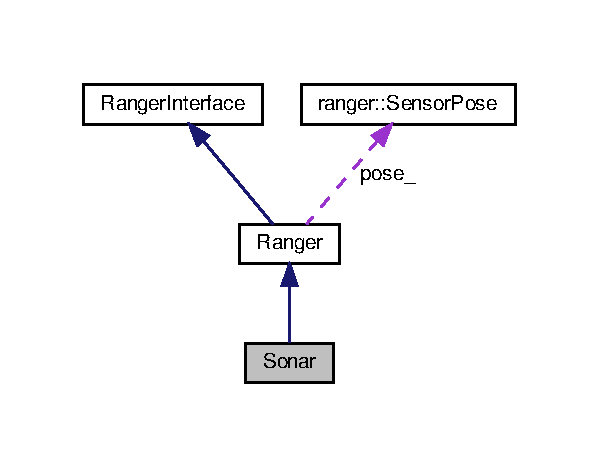
\includegraphics[width=288pt]{classSonar__coll__graph}
\end{center}
\end{figure}
\subsection*{Public Member Functions}
\begin{DoxyCompactItemize}
\item 
\mbox{\Hypertarget{classSonar_a16d2e4d63a621d350a0ae8b494f313ad}\label{classSonar_a16d2e4d63a621d350a0ae8b494f313ad}} 
void \hyperlink{classSonar_a16d2e4d63a621d350a0ae8b494f313ad}{get\+Set\+Params} (void)
\begin{DoxyCompactList}\small\item\em Prints out the parameters of the sensor that cannot be altered. \end{DoxyCompactList}\end{DoxyCompactItemize}
\subsection*{Additional Inherited Members}


The documentation for this class was generated from the following files\+:\begin{DoxyCompactItemize}
\item 
sonar.\+h\item 
sonar.\+cpp\end{DoxyCompactItemize}

\chapter{File Documentation}
\hypertarget{analysis_8h}{}\section{analysis.\+h File Reference}
\label{analysis_8h}\index{analysis.\+h@{analysis.\+h}}


The functions implemented to perform grabandfuse data function from rangerfusion along with caclulating the sonar union.  


{\ttfamily \#include $<$vector$>$}\newline
Include dependency graph for analysis.\+h\+:\nopagebreak
\begin{figure}[H]
\begin{center}
\leavevmode
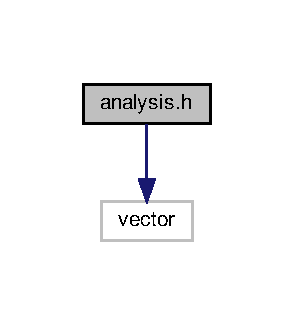
\includegraphics[width=141pt]{analysis_8h__incl}
\end{center}
\end{figure}
\subsection*{Classes}
\begin{DoxyCompactItemize}
\item 
struct \hyperlink{structgeometry__msgs_1_1Point}{geometry\+\_\+msgs\+::\+Point}
\end{DoxyCompactItemize}
\subsection*{Namespaces}
\begin{DoxyCompactItemize}
\item 
 \hyperlink{namespacegeometry__msgs}{geometry\+\_\+msgs}
\begin{DoxyCompactList}\small\item\em Analysis header. \end{DoxyCompactList}\end{DoxyCompactItemize}
\subsection*{Functions}
\begin{DoxyCompactItemize}
\item 
\hyperlink{structgeometry__msgs_1_1Point}{geometry\+\_\+msgs\+::\+Point} \hyperlink{analysis_8h_ae465d194c4c7840a63d5795d8ae228dd}{Pointof\+Line\+Intersection} (\hyperlink{structgeometry__msgs_1_1Point}{geometry\+\_\+msgs\+::\+Point} A, \hyperlink{structgeometry__msgs_1_1Point}{geometry\+\_\+msgs\+::\+Point} B, \hyperlink{structgeometry__msgs_1_1Point}{geometry\+\_\+msgs\+::\+Point} C, \hyperlink{structgeometry__msgs_1_1Point}{geometry\+\_\+msgs\+::\+Point} D)
\begin{DoxyCompactList}\small\item\em Finds the intersection points of two lines given by the points AB and CD. \end{DoxyCompactList}\item 
bool \hyperlink{analysis_8h_aa1d6670d93a84ed36cda29c39450a1f8}{Checkallsides} (\hyperlink{structgeometry__msgs_1_1Point}{geometry\+\_\+msgs\+::\+Point} a, \hyperlink{structgeometry__msgs_1_1Point}{geometry\+\_\+msgs\+::\+Point} b, \hyperlink{structgeometry__msgs_1_1Point}{geometry\+\_\+msgs\+::\+Point} c, \hyperlink{structgeometry__msgs_1_1Point}{geometry\+\_\+msgs\+::\+Point} a1, \hyperlink{structgeometry__msgs_1_1Point}{geometry\+\_\+msgs\+::\+Point} b1, \hyperlink{structgeometry__msgs_1_1Point}{geometry\+\_\+msgs\+::\+Point} c1, std\+::vector$<$ \hyperlink{structgeometry__msgs_1_1Point}{geometry\+\_\+msgs\+::\+Point} $>$ \&all\+\_\+\+P\+OI)
\begin{DoxyCompactList}\small\item\em Checks if any side of sonar i intersects with any sides of sonar i+1 by calling Pointof\+Line\+Intersection for each pair of sides (9 pairs) \end{DoxyCompactList}\item 
bool \hyperlink{analysis_8h_a0892990ee980096428256a73a16511eb}{is\+Inside\+Sonar} (\hyperlink{structgeometry__msgs_1_1Point}{geometry\+\_\+msgs\+::\+Point} sonar\+Start, \hyperlink{structgeometry__msgs_1_1Point}{geometry\+\_\+msgs\+::\+Point} sonar\+Corner1, \hyperlink{structgeometry__msgs_1_1Point}{geometry\+\_\+msgs\+::\+Point} sonar\+Corner2, \hyperlink{structgeometry__msgs_1_1Point}{geometry\+\_\+msgs\+::\+Point} a)
\begin{DoxyCompactList}\small\item\em Checks if any of the intersect points are inside the bounds of a sonar using Barycentric coordinate calculations. \end{DoxyCompactList}\item 
bool \hyperlink{analysis_8h_a04059a15651de8b2e18573e2d80e81a4}{Laser\+Intersect} (\hyperlink{structgeometry__msgs_1_1Point}{geometry\+\_\+msgs\+::\+Point} laser\+Start, \hyperlink{structgeometry__msgs_1_1Point}{geometry\+\_\+msgs\+::\+Point} laser\+End, \hyperlink{structgeometry__msgs_1_1Point}{geometry\+\_\+msgs\+::\+Point} a, \hyperlink{structgeometry__msgs_1_1Point}{geometry\+\_\+msgs\+::\+Point} b, \hyperlink{structgeometry__msgs_1_1Point}{geometry\+\_\+msgs\+::\+Point} c, \hyperlink{structgeometry__msgs_1_1Point}{geometry\+\_\+msgs\+::\+Point} d)
\begin{DoxyCompactList}\small\item\em Using the functions below, function determines if the line between the two laser points intersects with any of the cell edges defines by ab,bc,cd,da. \end{DoxyCompactList}\item 
bool \hyperlink{analysis_8h_a21bfb4cc97398db2005399cc44e241c8}{Sonar\+Occupied} (\hyperlink{structgeometry__msgs_1_1Point}{geometry\+\_\+msgs\+::\+Point} sonar\+Start, \hyperlink{structgeometry__msgs_1_1Point}{geometry\+\_\+msgs\+::\+Point} sonar\+Corner, double theta, double sonarangle, double radius, \hyperlink{structgeometry__msgs_1_1Point}{geometry\+\_\+msgs\+::\+Point} a, \hyperlink{structgeometry__msgs_1_1Point}{geometry\+\_\+msgs\+::\+Point} b, \hyperlink{structgeometry__msgs_1_1Point}{geometry\+\_\+msgs\+::\+Point} c, \hyperlink{structgeometry__msgs_1_1Point}{geometry\+\_\+msgs\+::\+Point} d)
\begin{DoxyCompactList}\small\item\em Establish a logic that if the sonar is to state a cell is O\+C\+C\+U\+P\+I\+ED, that the curve of the sonar, or the end of the cone M\+U\+ST then exist within the bounds of the cell. In this case, we implement a function in which it obtains points along the curve and checks if any of these points lie within a set margin around the cells edges. \end{DoxyCompactList}\item 
bool \hyperlink{analysis_8h_a07d7df90c424ace5027d3df90f391692}{Sonar\+Free} (double theta, double radius, double sonarangle, \hyperlink{structgeometry__msgs_1_1Point}{geometry\+\_\+msgs\+::\+Point} sonar\+Start, \hyperlink{structgeometry__msgs_1_1Point}{geometry\+\_\+msgs\+::\+Point} sonar\+Corner, \hyperlink{structgeometry__msgs_1_1Point}{geometry\+\_\+msgs\+::\+Point} a, \hyperlink{structgeometry__msgs_1_1Point}{geometry\+\_\+msgs\+::\+Point} b)
\begin{DoxyCompactList}\small\item\em Essentially, by converting the cell corner points into polar coordinates, a cell corner exists within the bounds of a sonar if the corner is a distance from the sonar start that is less than the sonar reading (radius) A\+ND the corner point is also within the 2 angle ranges from the positive x axis set by the 2 sonar edges E.\+g a sonar with 20 deg F\+OV facing forward along y axis would set angle bounds between 100 and 80 degrees If a cell corner exists W\+I\+T\+H\+IN the sonar bounds B\+UT is N\+OT found to be occupied it must then be F\+R\+EE. \end{DoxyCompactList}\item 
bool \hyperlink{analysis_8h_a129954038a3a9bb384bc48a70a817f22}{on\+Segment} (\hyperlink{structgeometry__msgs_1_1Point}{geometry\+\_\+msgs\+::\+Point} p, \hyperlink{structgeometry__msgs_1_1Point}{geometry\+\_\+msgs\+::\+Point} q, \hyperlink{structgeometry__msgs_1_1Point}{geometry\+\_\+msgs\+::\+Point} r)
\begin{DoxyCompactList}\small\item\em Given three colinear points p, q, r, the function checks if point q lies on line segment \textquotesingle{}pr\textquotesingle{}. \end{DoxyCompactList}\item 
double \hyperlink{analysis_8h_a58d731f1cd01e3cf2b75ed25500a23d9}{orientation} (\hyperlink{structgeometry__msgs_1_1Point}{geometry\+\_\+msgs\+::\+Point} p, \hyperlink{structgeometry__msgs_1_1Point}{geometry\+\_\+msgs\+::\+Point} q, \hyperlink{structgeometry__msgs_1_1Point}{geometry\+\_\+msgs\+::\+Point} r)
\begin{DoxyCompactList}\small\item\em To find orientation of ordered triplet (p, q, r). \end{DoxyCompactList}\item 
bool \hyperlink{analysis_8h_a89bd4ef12d2b7281c3a2b9b819d330be}{do\+Intersect} (\hyperlink{structgeometry__msgs_1_1Point}{geometry\+\_\+msgs\+::\+Point} p1, \hyperlink{structgeometry__msgs_1_1Point}{geometry\+\_\+msgs\+::\+Point} q1, \hyperlink{structgeometry__msgs_1_1Point}{geometry\+\_\+msgs\+::\+Point} p2, \hyperlink{structgeometry__msgs_1_1Point}{geometry\+\_\+msgs\+::\+Point} q2)
\begin{DoxyCompactList}\small\item\em Function that returns true if line segment \textquotesingle{}p1q1\textquotesingle{} intersects \textquotesingle{}p2q2\textquotesingle{}. \end{DoxyCompactList}\end{DoxyCompactItemize}


\subsection{Detailed Description}
The functions implemented to perform grabandfuse data function from rangerfusion along with caclulating the sonar union. 



\subsection{Function Documentation}
\mbox{\Hypertarget{analysis_8h_aa1d6670d93a84ed36cda29c39450a1f8}\label{analysis_8h_aa1d6670d93a84ed36cda29c39450a1f8}} 
\index{analysis.\+h@{analysis.\+h}!Checkallsides@{Checkallsides}}
\index{Checkallsides@{Checkallsides}!analysis.\+h@{analysis.\+h}}
\subsubsection{\texorpdfstring{Checkallsides()}{Checkallsides()}}
{\footnotesize\ttfamily bool Checkallsides (\begin{DoxyParamCaption}\item[{\hyperlink{structgeometry__msgs_1_1Point}{geometry\+\_\+msgs\+::\+Point}}]{a,  }\item[{\hyperlink{structgeometry__msgs_1_1Point}{geometry\+\_\+msgs\+::\+Point}}]{b,  }\item[{\hyperlink{structgeometry__msgs_1_1Point}{geometry\+\_\+msgs\+::\+Point}}]{c,  }\item[{\hyperlink{structgeometry__msgs_1_1Point}{geometry\+\_\+msgs\+::\+Point}}]{a1,  }\item[{\hyperlink{structgeometry__msgs_1_1Point}{geometry\+\_\+msgs\+::\+Point}}]{b1,  }\item[{\hyperlink{structgeometry__msgs_1_1Point}{geometry\+\_\+msgs\+::\+Point}}]{c1,  }\item[{std\+::vector$<$ \hyperlink{structgeometry__msgs_1_1Point}{geometry\+\_\+msgs\+::\+Point} $>$ \&}]{all\+\_\+\+P\+OI }\end{DoxyParamCaption})}



Checks if any side of sonar i intersects with any sides of sonar i+1 by calling Pointof\+Line\+Intersection for each pair of sides (9 pairs) 


\begin{DoxyParams}{Parameters}
{\em a} & 3 sides of sonar i \\
\hline
{\em b} & \\
\hline
{\em c} & \\
\hline
{\em a1} & 3 sides of sonar i+1 \\
\hline
{\em b1} & \\
\hline
{\em c1} & \\
\hline
{\em all\+\_\+\+P\+OI} & vector containing all points of intersection \\
\hline
\end{DoxyParams}
\begin{DoxyReturn}{Returns}
true returns true to indicate that the sonar does intersect with another sonar 

false returns false to indicate that the sonar does N\+OT intersect with another sonar 
\end{DoxyReturn}
\mbox{\Hypertarget{analysis_8h_a89bd4ef12d2b7281c3a2b9b819d330be}\label{analysis_8h_a89bd4ef12d2b7281c3a2b9b819d330be}} 
\index{analysis.\+h@{analysis.\+h}!do\+Intersect@{do\+Intersect}}
\index{do\+Intersect@{do\+Intersect}!analysis.\+h@{analysis.\+h}}
\subsubsection{\texorpdfstring{do\+Intersect()}{doIntersect()}}
{\footnotesize\ttfamily bool do\+Intersect (\begin{DoxyParamCaption}\item[{\hyperlink{structgeometry__msgs_1_1Point}{geometry\+\_\+msgs\+::\+Point}}]{p1,  }\item[{\hyperlink{structgeometry__msgs_1_1Point}{geometry\+\_\+msgs\+::\+Point}}]{q1,  }\item[{\hyperlink{structgeometry__msgs_1_1Point}{geometry\+\_\+msgs\+::\+Point}}]{p2,  }\item[{\hyperlink{structgeometry__msgs_1_1Point}{geometry\+\_\+msgs\+::\+Point}}]{q2 }\end{DoxyParamCaption})}



Function that returns true if line segment \textquotesingle{}p1q1\textquotesingle{} intersects \textquotesingle{}p2q2\textquotesingle{}. 


\begin{DoxyParams}{Parameters}
{\em p1} & first point of line 1 \\
\hline
{\em q1} & second point of line 1 \\
\hline
{\em p2} & first point of line 2 \\
\hline
{\em q2} & second point of line 2 \\
\hline
\end{DoxyParams}
\begin{DoxyReturn}{Returns}
boolean indicating lines intersect 
\end{DoxyReturn}
\begin{DoxyNote}{Note}
atttribution to \href{https://www.geeksforgeeks.org/check-if-two-given-line-segments-intersect/}{\tt https\+://www.\+geeksforgeeks.\+org/check-\/if-\/two-\/given-\/line-\/segments-\/intersect/} 
\end{DoxyNote}
\mbox{\Hypertarget{analysis_8h_a0892990ee980096428256a73a16511eb}\label{analysis_8h_a0892990ee980096428256a73a16511eb}} 
\index{analysis.\+h@{analysis.\+h}!is\+Inside\+Sonar@{is\+Inside\+Sonar}}
\index{is\+Inside\+Sonar@{is\+Inside\+Sonar}!analysis.\+h@{analysis.\+h}}
\subsubsection{\texorpdfstring{is\+Inside\+Sonar()}{isInsideSonar()}}
{\footnotesize\ttfamily bool is\+Inside\+Sonar (\begin{DoxyParamCaption}\item[{\hyperlink{structgeometry__msgs_1_1Point}{geometry\+\_\+msgs\+::\+Point}}]{sonar\+Start,  }\item[{\hyperlink{structgeometry__msgs_1_1Point}{geometry\+\_\+msgs\+::\+Point}}]{sonar\+Corner1,  }\item[{\hyperlink{structgeometry__msgs_1_1Point}{geometry\+\_\+msgs\+::\+Point}}]{sonar\+Corner2,  }\item[{\hyperlink{structgeometry__msgs_1_1Point}{geometry\+\_\+msgs\+::\+Point}}]{a }\end{DoxyParamCaption})}



Checks if any of the intersect points are inside the bounds of a sonar using Barycentric coordinate calculations. 


\begin{DoxyParams}{Parameters}
{\em sonar\+Start} & \\
\hline
{\em sonar\+Corner1} & \\
\hline
{\em sonar\+Corner2} & \\
\hline
{\em a} & \\
\hline
\end{DoxyParams}
\begin{DoxyReturn}{Returns}
true 

false 
\end{DoxyReturn}
\mbox{\Hypertarget{analysis_8h_a04059a15651de8b2e18573e2d80e81a4}\label{analysis_8h_a04059a15651de8b2e18573e2d80e81a4}} 
\index{analysis.\+h@{analysis.\+h}!Laser\+Intersect@{Laser\+Intersect}}
\index{Laser\+Intersect@{Laser\+Intersect}!analysis.\+h@{analysis.\+h}}
\subsubsection{\texorpdfstring{Laser\+Intersect()}{LaserIntersect()}}
{\footnotesize\ttfamily bool Laser\+Intersect (\begin{DoxyParamCaption}\item[{\hyperlink{structgeometry__msgs_1_1Point}{geometry\+\_\+msgs\+::\+Point}}]{laser\+Start,  }\item[{\hyperlink{structgeometry__msgs_1_1Point}{geometry\+\_\+msgs\+::\+Point}}]{laser\+End,  }\item[{\hyperlink{structgeometry__msgs_1_1Point}{geometry\+\_\+msgs\+::\+Point}}]{a,  }\item[{\hyperlink{structgeometry__msgs_1_1Point}{geometry\+\_\+msgs\+::\+Point}}]{b,  }\item[{\hyperlink{structgeometry__msgs_1_1Point}{geometry\+\_\+msgs\+::\+Point}}]{c,  }\item[{\hyperlink{structgeometry__msgs_1_1Point}{geometry\+\_\+msgs\+::\+Point}}]{d }\end{DoxyParamCaption})}



Using the functions below, function determines if the line between the two laser points intersects with any of the cell edges defines by ab,bc,cd,da. 


\begin{DoxyParams}{Parameters}
{\em laser\+Start} & \\
\hline
{\em laser\+End} & \\
\hline
{\em a} & \\
\hline
{\em b} & \\
\hline
{\em c} & \\
\hline
{\em d} & \\
\hline
\end{DoxyParams}
\begin{DoxyReturn}{Returns}
true 

false 
\end{DoxyReturn}
\mbox{\Hypertarget{analysis_8h_a129954038a3a9bb384bc48a70a817f22}\label{analysis_8h_a129954038a3a9bb384bc48a70a817f22}} 
\index{analysis.\+h@{analysis.\+h}!on\+Segment@{on\+Segment}}
\index{on\+Segment@{on\+Segment}!analysis.\+h@{analysis.\+h}}
\subsubsection{\texorpdfstring{on\+Segment()}{onSegment()}}
{\footnotesize\ttfamily bool on\+Segment (\begin{DoxyParamCaption}\item[{\hyperlink{structgeometry__msgs_1_1Point}{geometry\+\_\+msgs\+::\+Point}}]{p,  }\item[{\hyperlink{structgeometry__msgs_1_1Point}{geometry\+\_\+msgs\+::\+Point}}]{q,  }\item[{\hyperlink{structgeometry__msgs_1_1Point}{geometry\+\_\+msgs\+::\+Point}}]{r }\end{DoxyParamCaption})}



Given three colinear points p, q, r, the function checks if point q lies on line segment \textquotesingle{}pr\textquotesingle{}. 


\begin{DoxyParams}{Parameters}
{\em p} & colinear point \\
\hline
{\em q} & colinear point \\
\hline
{\em r} & colinear point \\
\hline
\end{DoxyParams}
\begin{DoxyReturn}{Returns}
boolean indicating point q lies on line segment \textquotesingle{}pr\textquotesingle{} 
\end{DoxyReturn}
\begin{DoxyNote}{Note}
atttribution to \href{https://www.geeksforgeeks.org/check-if-two-given-line-segments-intersect/}{\tt https\+://www.\+geeksforgeeks.\+org/check-\/if-\/two-\/given-\/line-\/segments-\/intersect/} 
\end{DoxyNote}
\mbox{\Hypertarget{analysis_8h_a58d731f1cd01e3cf2b75ed25500a23d9}\label{analysis_8h_a58d731f1cd01e3cf2b75ed25500a23d9}} 
\index{analysis.\+h@{analysis.\+h}!orientation@{orientation}}
\index{orientation@{orientation}!analysis.\+h@{analysis.\+h}}
\subsubsection{\texorpdfstring{orientation()}{orientation()}}
{\footnotesize\ttfamily double orientation (\begin{DoxyParamCaption}\item[{\hyperlink{structgeometry__msgs_1_1Point}{geometry\+\_\+msgs\+::\+Point}}]{p,  }\item[{\hyperlink{structgeometry__msgs_1_1Point}{geometry\+\_\+msgs\+::\+Point}}]{q,  }\item[{\hyperlink{structgeometry__msgs_1_1Point}{geometry\+\_\+msgs\+::\+Point}}]{r }\end{DoxyParamCaption})}



To find orientation of ordered triplet (p, q, r). 


\begin{DoxyParams}{Parameters}
{\em p} & point \\
\hline
{\em q} & point \\
\hline
{\em r} & point \\
\hline
\end{DoxyParams}
\begin{DoxyReturn}{Returns}
boolean 0 --$>$ p, q and r are colinear 1 --$>$ Clockwise 2 --$>$ Counterclockwise 
\end{DoxyReturn}
\begin{DoxyNote}{Note}
atttribution to \href{https://www.geeksforgeeks.org/check-if-two-given-line-segments-intersect/}{\tt https\+://www.\+geeksforgeeks.\+org/check-\/if-\/two-\/given-\/line-\/segments-\/intersect/} 
\end{DoxyNote}
\mbox{\Hypertarget{analysis_8h_ae465d194c4c7840a63d5795d8ae228dd}\label{analysis_8h_ae465d194c4c7840a63d5795d8ae228dd}} 
\index{analysis.\+h@{analysis.\+h}!Pointof\+Line\+Intersection@{Pointof\+Line\+Intersection}}
\index{Pointof\+Line\+Intersection@{Pointof\+Line\+Intersection}!analysis.\+h@{analysis.\+h}}
\subsubsection{\texorpdfstring{Pointof\+Line\+Intersection()}{PointofLineIntersection()}}
{\footnotesize\ttfamily \hyperlink{structgeometry__msgs_1_1Point}{geometry\+\_\+msgs\+::\+Point} Pointof\+Line\+Intersection (\begin{DoxyParamCaption}\item[{\hyperlink{structgeometry__msgs_1_1Point}{geometry\+\_\+msgs\+::\+Point}}]{A,  }\item[{\hyperlink{structgeometry__msgs_1_1Point}{geometry\+\_\+msgs\+::\+Point}}]{B,  }\item[{\hyperlink{structgeometry__msgs_1_1Point}{geometry\+\_\+msgs\+::\+Point}}]{C,  }\item[{\hyperlink{structgeometry__msgs_1_1Point}{geometry\+\_\+msgs\+::\+Point}}]{D }\end{DoxyParamCaption})}



Finds the intersection points of two lines given by the points AB and CD. 


\begin{DoxyParams}{Parameters}
{\em A} & \\
\hline
{\em B} & \\
\hline
{\em C} & \\
\hline
{\em D} & \\
\hline
\end{DoxyParams}
\begin{DoxyReturn}{Returns}
\hyperlink{structgeometry__msgs_1_1Point}{geometry\+\_\+msgs\+::\+Point} intersection points 
\end{DoxyReturn}
\mbox{\Hypertarget{analysis_8h_a07d7df90c424ace5027d3df90f391692}\label{analysis_8h_a07d7df90c424ace5027d3df90f391692}} 
\index{analysis.\+h@{analysis.\+h}!Sonar\+Free@{Sonar\+Free}}
\index{Sonar\+Free@{Sonar\+Free}!analysis.\+h@{analysis.\+h}}
\subsubsection{\texorpdfstring{Sonar\+Free()}{SonarFree()}}
{\footnotesize\ttfamily bool Sonar\+Free (\begin{DoxyParamCaption}\item[{double}]{theta,  }\item[{double}]{radius,  }\item[{double}]{sonarangle,  }\item[{\hyperlink{structgeometry__msgs_1_1Point}{geometry\+\_\+msgs\+::\+Point}}]{sonar\+Start,  }\item[{\hyperlink{structgeometry__msgs_1_1Point}{geometry\+\_\+msgs\+::\+Point}}]{sonar\+Corner,  }\item[{\hyperlink{structgeometry__msgs_1_1Point}{geometry\+\_\+msgs\+::\+Point}}]{a,  }\item[{\hyperlink{structgeometry__msgs_1_1Point}{geometry\+\_\+msgs\+::\+Point}}]{b }\end{DoxyParamCaption})}



Essentially, by converting the cell corner points into polar coordinates, a cell corner exists within the bounds of a sonar if the corner is a distance from the sonar start that is less than the sonar reading (radius) A\+ND the corner point is also within the 2 angle ranges from the positive x axis set by the 2 sonar edges E.\+g a sonar with 20 deg F\+OV facing forward along y axis would set angle bounds between 100 and 80 degrees If a cell corner exists W\+I\+T\+H\+IN the sonar bounds B\+UT is N\+OT found to be occupied it must then be F\+R\+EE. 


\begin{DoxyParams}{Parameters}
{\em theta} & \\
\hline
{\em radius} & \\
\hline
{\em sonarangle} & \\
\hline
{\em sonar\+Start} & \\
\hline
{\em sonar\+Corner} & \\
\hline
{\em a} & \\
\hline
{\em b} & \\
\hline
\end{DoxyParams}
\begin{DoxyReturn}{Returns}
true 

false 
\end{DoxyReturn}
\mbox{\Hypertarget{analysis_8h_a21bfb4cc97398db2005399cc44e241c8}\label{analysis_8h_a21bfb4cc97398db2005399cc44e241c8}} 
\index{analysis.\+h@{analysis.\+h}!Sonar\+Occupied@{Sonar\+Occupied}}
\index{Sonar\+Occupied@{Sonar\+Occupied}!analysis.\+h@{analysis.\+h}}
\subsubsection{\texorpdfstring{Sonar\+Occupied()}{SonarOccupied()}}
{\footnotesize\ttfamily bool Sonar\+Occupied (\begin{DoxyParamCaption}\item[{\hyperlink{structgeometry__msgs_1_1Point}{geometry\+\_\+msgs\+::\+Point}}]{sonar\+Start,  }\item[{\hyperlink{structgeometry__msgs_1_1Point}{geometry\+\_\+msgs\+::\+Point}}]{sonar\+Corner,  }\item[{double}]{theta,  }\item[{double}]{sonarangle,  }\item[{double}]{radius,  }\item[{\hyperlink{structgeometry__msgs_1_1Point}{geometry\+\_\+msgs\+::\+Point}}]{a,  }\item[{\hyperlink{structgeometry__msgs_1_1Point}{geometry\+\_\+msgs\+::\+Point}}]{b,  }\item[{\hyperlink{structgeometry__msgs_1_1Point}{geometry\+\_\+msgs\+::\+Point}}]{c,  }\item[{\hyperlink{structgeometry__msgs_1_1Point}{geometry\+\_\+msgs\+::\+Point}}]{d }\end{DoxyParamCaption})}



Establish a logic that if the sonar is to state a cell is O\+C\+C\+U\+P\+I\+ED, that the curve of the sonar, or the end of the cone M\+U\+ST then exist within the bounds of the cell. In this case, we implement a function in which it obtains points along the curve and checks if any of these points lie within a set margin around the cells edges. 


\begin{DoxyParams}{Parameters}
{\em sonar\+Start} & \\
\hline
{\em sonar\+Corner} & \\
\hline
{\em a} & top left corner \\
\hline
{\em b} & bottom left corner \\
\hline
{\em c} & bottom right corner \\
\hline
{\em d} & top right corner \\
\hline
\end{DoxyParams}
\begin{DoxyReturn}{Returns}
true 

false 
\end{DoxyReturn}

%--- End generated contents ---

% Index
\backmatter
\newpage
\phantomsection
\clearemptydoublepage
\addcontentsline{toc}{chapter}{Index}
\printindex

\end{document}
